\documentclass[12pt,]{book}
\usepackage{lmodern}
\usepackage{amssymb,amsmath}
\usepackage{ifxetex,ifluatex}
\usepackage{fixltx2e} % provides \textsubscript
\ifnum 0\ifxetex 1\fi\ifluatex 1\fi=0 % if pdftex
  \usepackage[T1]{fontenc}
  \usepackage[utf8]{inputenc}
\else % if luatex or xelatex
  \ifxetex
    \usepackage{mathspec}
  \else
    \usepackage{fontspec}
  \fi
  \defaultfontfeatures{Ligatures=TeX,Scale=MatchLowercase}
\fi
% use upquote if available, for straight quotes in verbatim environments
\IfFileExists{upquote.sty}{\usepackage{upquote}}{}
% use microtype if available
\IfFileExists{microtype.sty}{%
\usepackage{microtype}
\UseMicrotypeSet[protrusion]{basicmath} % disable protrusion for tt fonts
}{}
\usepackage[margin=1in]{geometry}
\usepackage{hyperref}
\PassOptionsToPackage{usenames,dvipsnames}{color} % color is loaded by hyperref
\hypersetup{unicode=true,
            pdftitle={AllCCS Tutorial V1.00},
            pdfauthor={Zhiwei Zhou},
            colorlinks=true,
            linkcolor=Maroon,
            citecolor=Blue,
            urlcolor=Blue,
            breaklinks=true}
\urlstyle{same}  % don't use monospace font for urls
\usepackage{natbib}
\bibliographystyle{apalike}
\usepackage{longtable,booktabs}
\usepackage{graphicx,grffile}
\makeatletter
\def\maxwidth{\ifdim\Gin@nat@width>\linewidth\linewidth\else\Gin@nat@width\fi}
\def\maxheight{\ifdim\Gin@nat@height>\textheight\textheight\else\Gin@nat@height\fi}
\makeatother
% Scale images if necessary, so that they will not overflow the page
% margins by default, and it is still possible to overwrite the defaults
% using explicit options in \includegraphics[width, height, ...]{}
\setkeys{Gin}{width=\maxwidth,height=\maxheight,keepaspectratio}
\IfFileExists{parskip.sty}{%
\usepackage{parskip}
}{% else
\setlength{\parindent}{0pt}
\setlength{\parskip}{6pt plus 2pt minus 1pt}
}
\setlength{\emergencystretch}{3em}  % prevent overfull lines
\providecommand{\tightlist}{%
  \setlength{\itemsep}{0pt}\setlength{\parskip}{0pt}}
\setcounter{secnumdepth}{5}
% Redefines (sub)paragraphs to behave more like sections
\ifx\paragraph\undefined\else
\let\oldparagraph\paragraph
\renewcommand{\paragraph}[1]{\oldparagraph{#1}\mbox{}}
\fi
\ifx\subparagraph\undefined\else
\let\oldsubparagraph\subparagraph
\renewcommand{\subparagraph}[1]{\oldsubparagraph{#1}\mbox{}}
\fi

%%% Use protect on footnotes to avoid problems with footnotes in titles
\let\rmarkdownfootnote\footnote%
\def\footnote{\protect\rmarkdownfootnote}

%%% Change title format to be more compact
\usepackage{titling}

% Create subtitle command for use in maketitle
\newcommand{\subtitle}[1]{
  \posttitle{
    \begin{center}\large#1\end{center}
    }
}

\setlength{\droptitle}{-2em}

  \title{AllCCS Tutorial V1.00}
    \pretitle{\vspace{\droptitle}\centering\huge}
  \posttitle{\par}
    \author{Zhiwei Zhou}
    \preauthor{\centering\large\emph}
  \postauthor{\par}
      \predate{\centering\large\emph}
  \postdate{\par}
    \date{2019-11-01}

\usepackage{booktabs}

\usepackage{amsthm}
\newtheorem{theorem}{Theorem}[chapter]
\newtheorem{lemma}{Lemma}[chapter]
\theoremstyle{definition}
\newtheorem{definition}{Definition}[chapter]
\newtheorem{corollary}{Corollary}[chapter]
\newtheorem{proposition}{Proposition}[chapter]
\theoremstyle{definition}
\newtheorem{example}{Example}[chapter]
\theoremstyle{definition}
\newtheorem{exercise}{Exercise}[chapter]
\theoremstyle{remark}
\newtheorem*{remark}{Remark}
\newtheorem*{solution}{Solution}
\begin{document}
\maketitle

{
\hypersetup{linkcolor=black}
\setcounter{tocdepth}{1}
\tableofcontents
}
\listoftables
\listoffigures
\chapter*{About AllCCS}\label{about-allccs}
\addcontentsline{toc}{chapter}{About AllCCS}

Copyright (c) 2019 AllCCS Development Team

\href{http://allccs.zhulab.cn/}{\textbf{AllCCS}} is a powerful platform
to support various applications in Ion Mobility -- Mass Spectrometry
(IM-MS). It is designed to contain three major parts: \textbf{1) Unified
CCS database, 2) Machine learning based CCS prediction, and 3) small
molecule annotation}. The unified CCS database is one of the most
comprehensive CCS databases, covering \textasciitilde{}1,700,000 small
molecules. It provides a universal platform to contain both experimental
CCS values (3,539) and predicted CCS values (over 10,000,000). Machine
learning based CCS prediction function supports convenient prediction
from SMILES structure to CCS values. This function utilizes the second
generation CCS prediction algorithm to generate CCS values and RSS score
for novel structures. Small molecule annotation provides an easy-to-use
annotation function for various features or compounds. It is supported
to search database with measured m/z and CCS for annotation, or in
conjunct with any other annotation tools, such as MetFrag, CFM-ID,
MS-Finder, and SIRUS etc.

Zhiwei Zhou (\url{zhouzw@sioc.ac.cn}) Zheng-Jiang Zhu
(\url{jiangzhu@sioc.ac.cn}) \href{http://www.zhulab.cn/}{Laboratory for
Mass Spectrometry and Metabolomics}
\href{http://www.ircbc.ac.cn/}{IRCBC}, Shanghai Institute of Organic
Chemistry Chinese Academy of Sciences, Shanghai, China

\chapter*{Citation}\label{citation}
\addcontentsline{toc}{chapter}{Citation}

If AllCCS is useful in your project, please cite our articles.

\begin{itemize}
\tightlist
\item
  Z. Zhou, Z.-J. Zhu* etc. Advancing CCS database towards metabolite
  annotation, In preparing
\end{itemize}

\chapter*{News}\label{news}
\addcontentsline{toc}{chapter}{News}

\textbf{December 1, 2019}

\begin{itemize}
\tightlist
\item
  Add reference for tutorial
\end{itemize}

\textbf{November 25, 2019}

\begin{itemize}
\tightlist
\item
  Update tutorial
\item
  Fix some known problems
\end{itemize}

\textbf{November 6, 2019}

\begin{itemize}
\tightlist
\item
  Test in web server
\item
  Fix bugs in admin system
\item
  Fix some known bugs
\item
  Update formal database and install AllCCS package V0.1.61
\item
  Correct compound name of drugbank compound 
\end{itemize}

\textbf{September 22, 2019}

\begin{itemize}
\tightlist
\item
  Demo webserver online
\end{itemize}

\chapter{Quick Start Guide}\label{chapter1}

\section{Create a AllCCS account}\label{chaptere1d1}

Users need to register AllCCS account to use the webserver. This process
is very sample, and \textbf{completely private}. To register an account,
navigate to the home page. The ``Sign up'' button is in the upper right
corner of the page. Then, you need to fill in your email and
verification code which would be sent to your email (Figure
\ref{fig:FigRegister}). Finally, input some basic information to
complete the registration. You could log in and enjoy all functions in
the web server.

\begin{figure}

{\centering 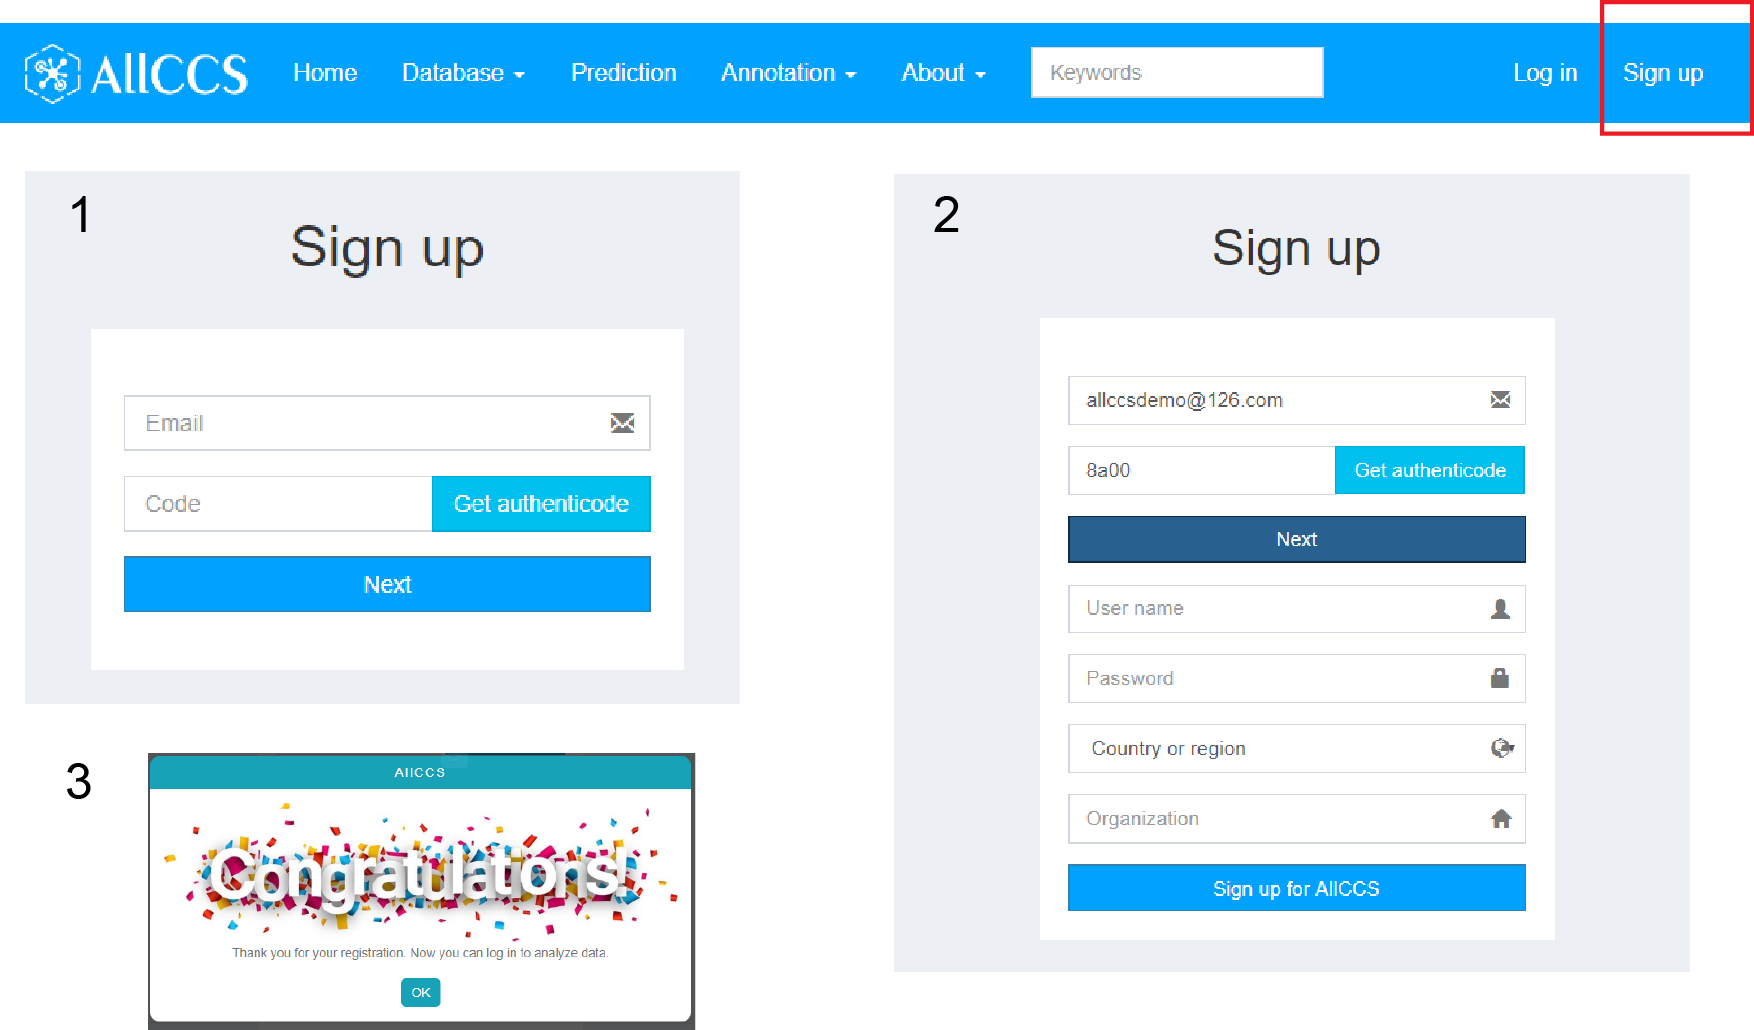
\includegraphics{images/chapter1/register_1} 

}

\caption{Register AllCCS account}\label{fig:FigRegister}
\end{figure}

\section{Browser CCS database}\label{chaptere1d2}

You could search you interested compound (name, formula, smiles, inchi,
InChIKey etc.) in the search box in navigation bar, or directly browser
the all database records in the ``browser'' page (Figure
\ref{fig:FigBrowser1}).

\begin{figure}

{\centering 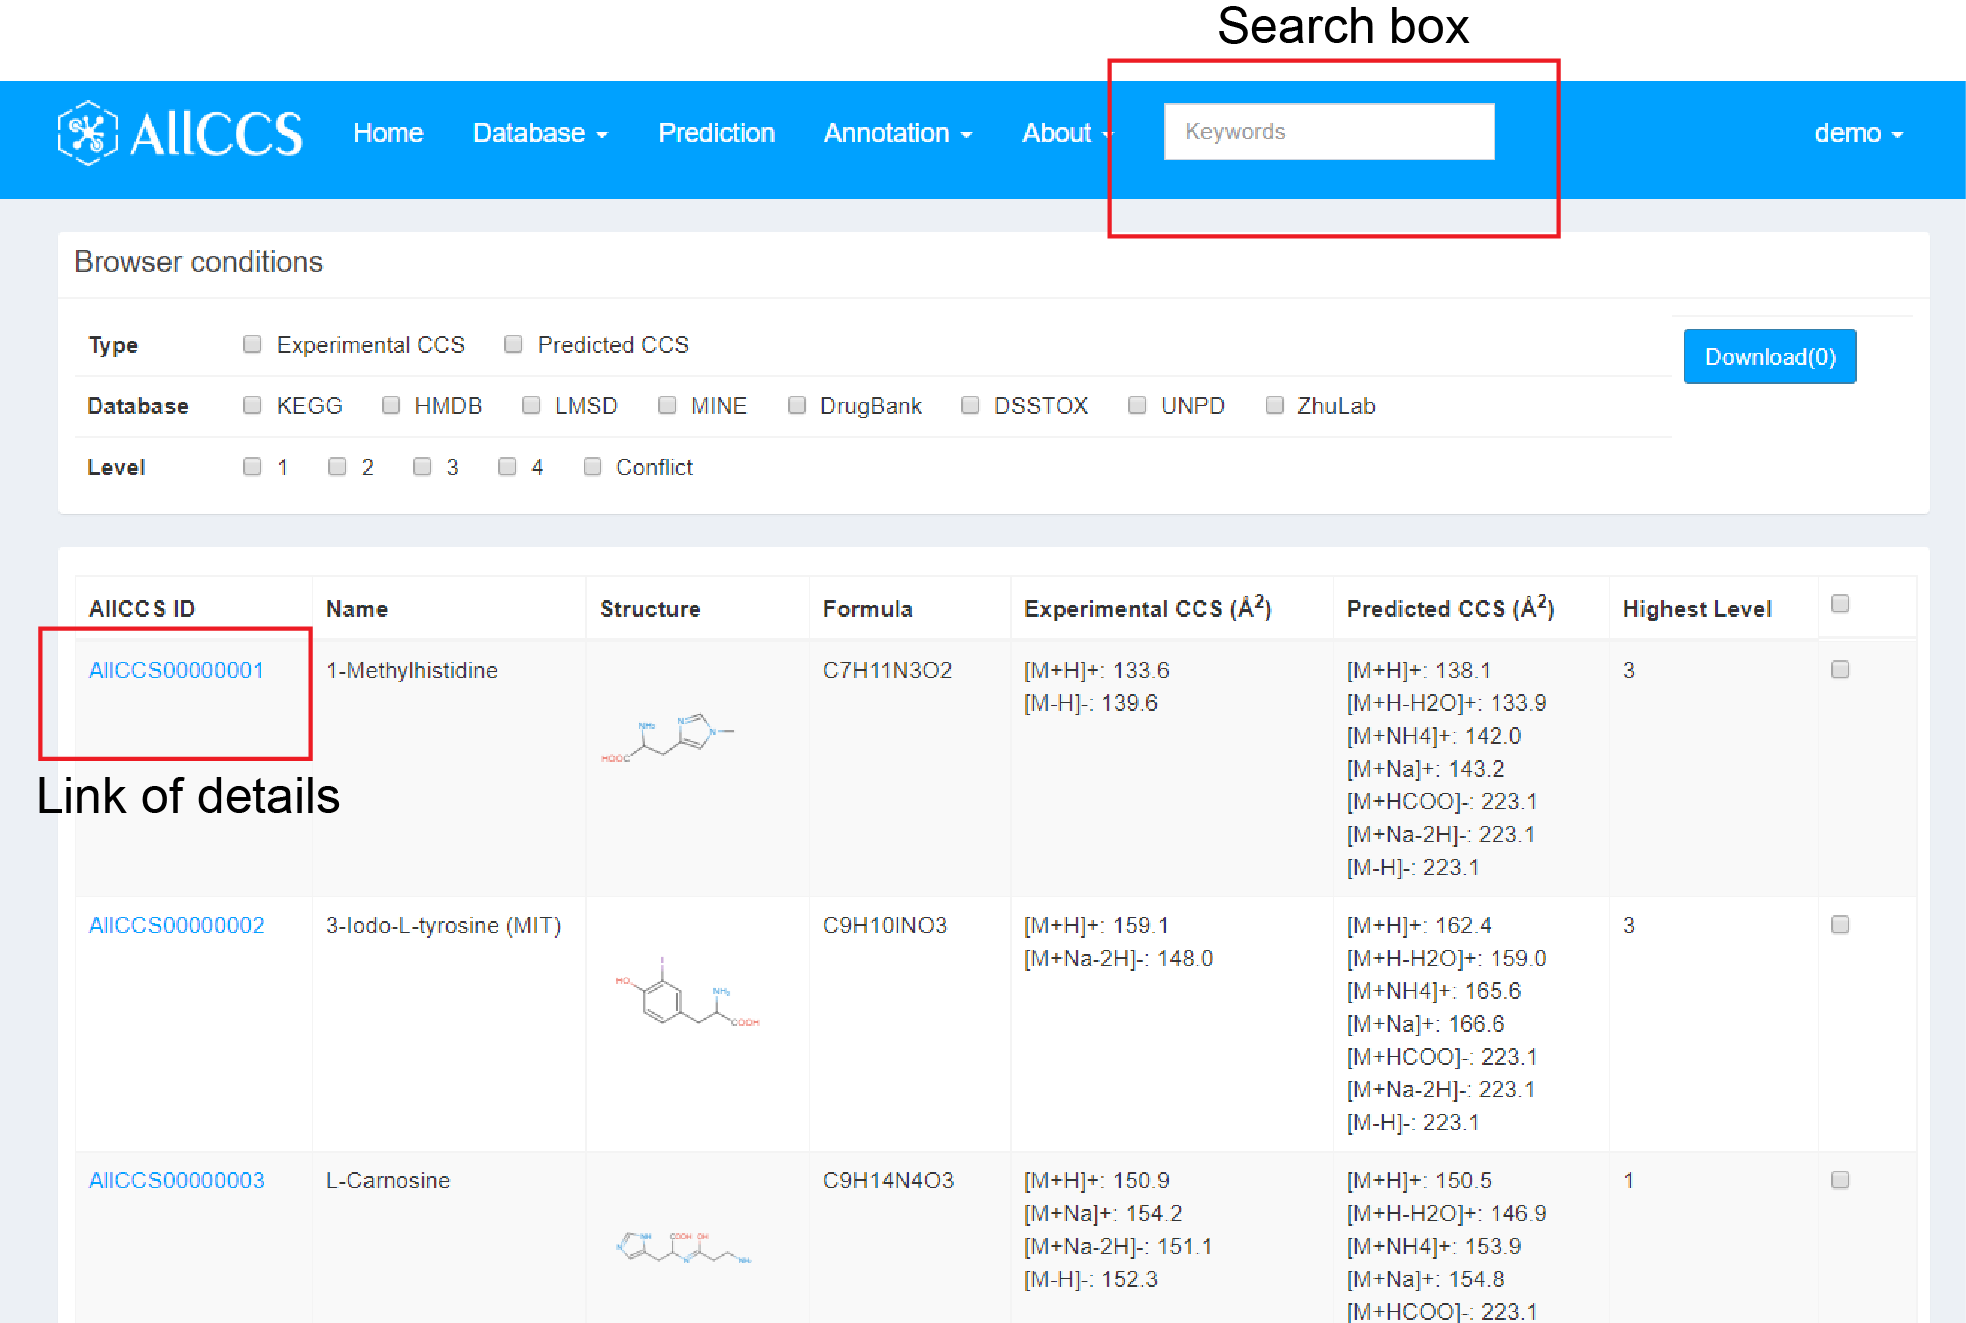
\includegraphics{images/chapter1/browser_1} 

}

\caption{Browser CCS database}\label{fig:FigBrowser1}
\end{figure}

Then, you can click the link in the column of AllCCS ID to browser
detail information of this compound (Figure \ref{fig:FigBrowser2}). It
includes basic meta information, unified CCS values, experimental CCS
records, predicted CCS records and other database links etc. Please see
section \ref{chapter2} for more details.

\begin{figure}

{\centering 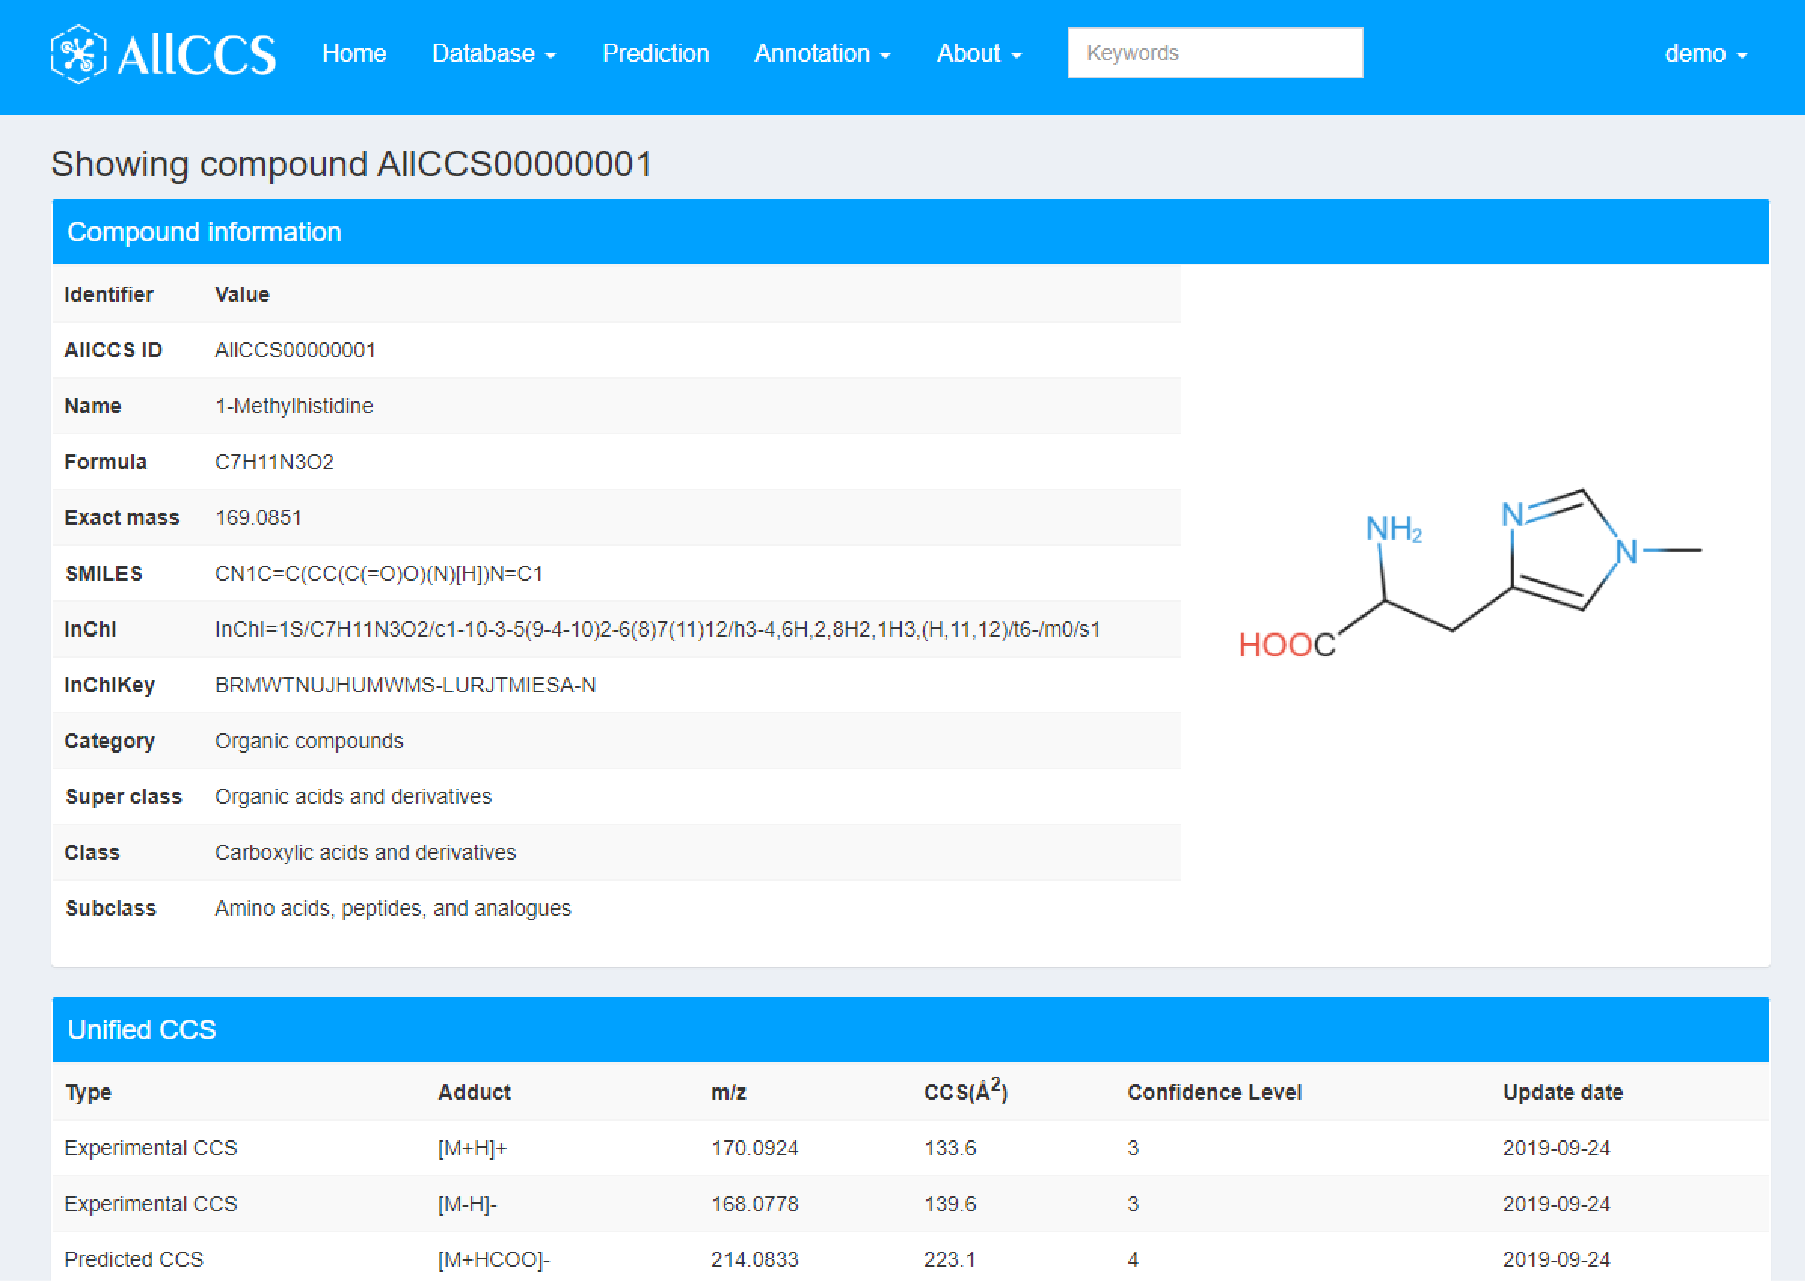
\includegraphics{images/chapter1/browser_2} 

}

\caption{Details of compounds}\label{fig:FigBrowser2}
\end{figure}

\section{Perform CCS prediction/annotation}\label{chaptere1d3}

AllCCS also provides CCS prediction function (Section \ref{chapter3})
and metabolite annotation functions (Section \ref{chapter4}). You could
click the link or corresponding item in navigation bar. For CCS
prediction function, please input the SMILES list of your compounds in
the input panel. The result would be returned on the project panel
within several seconds (Figure \ref{fig:FigPrediction}).

\begin{figure}

{\centering 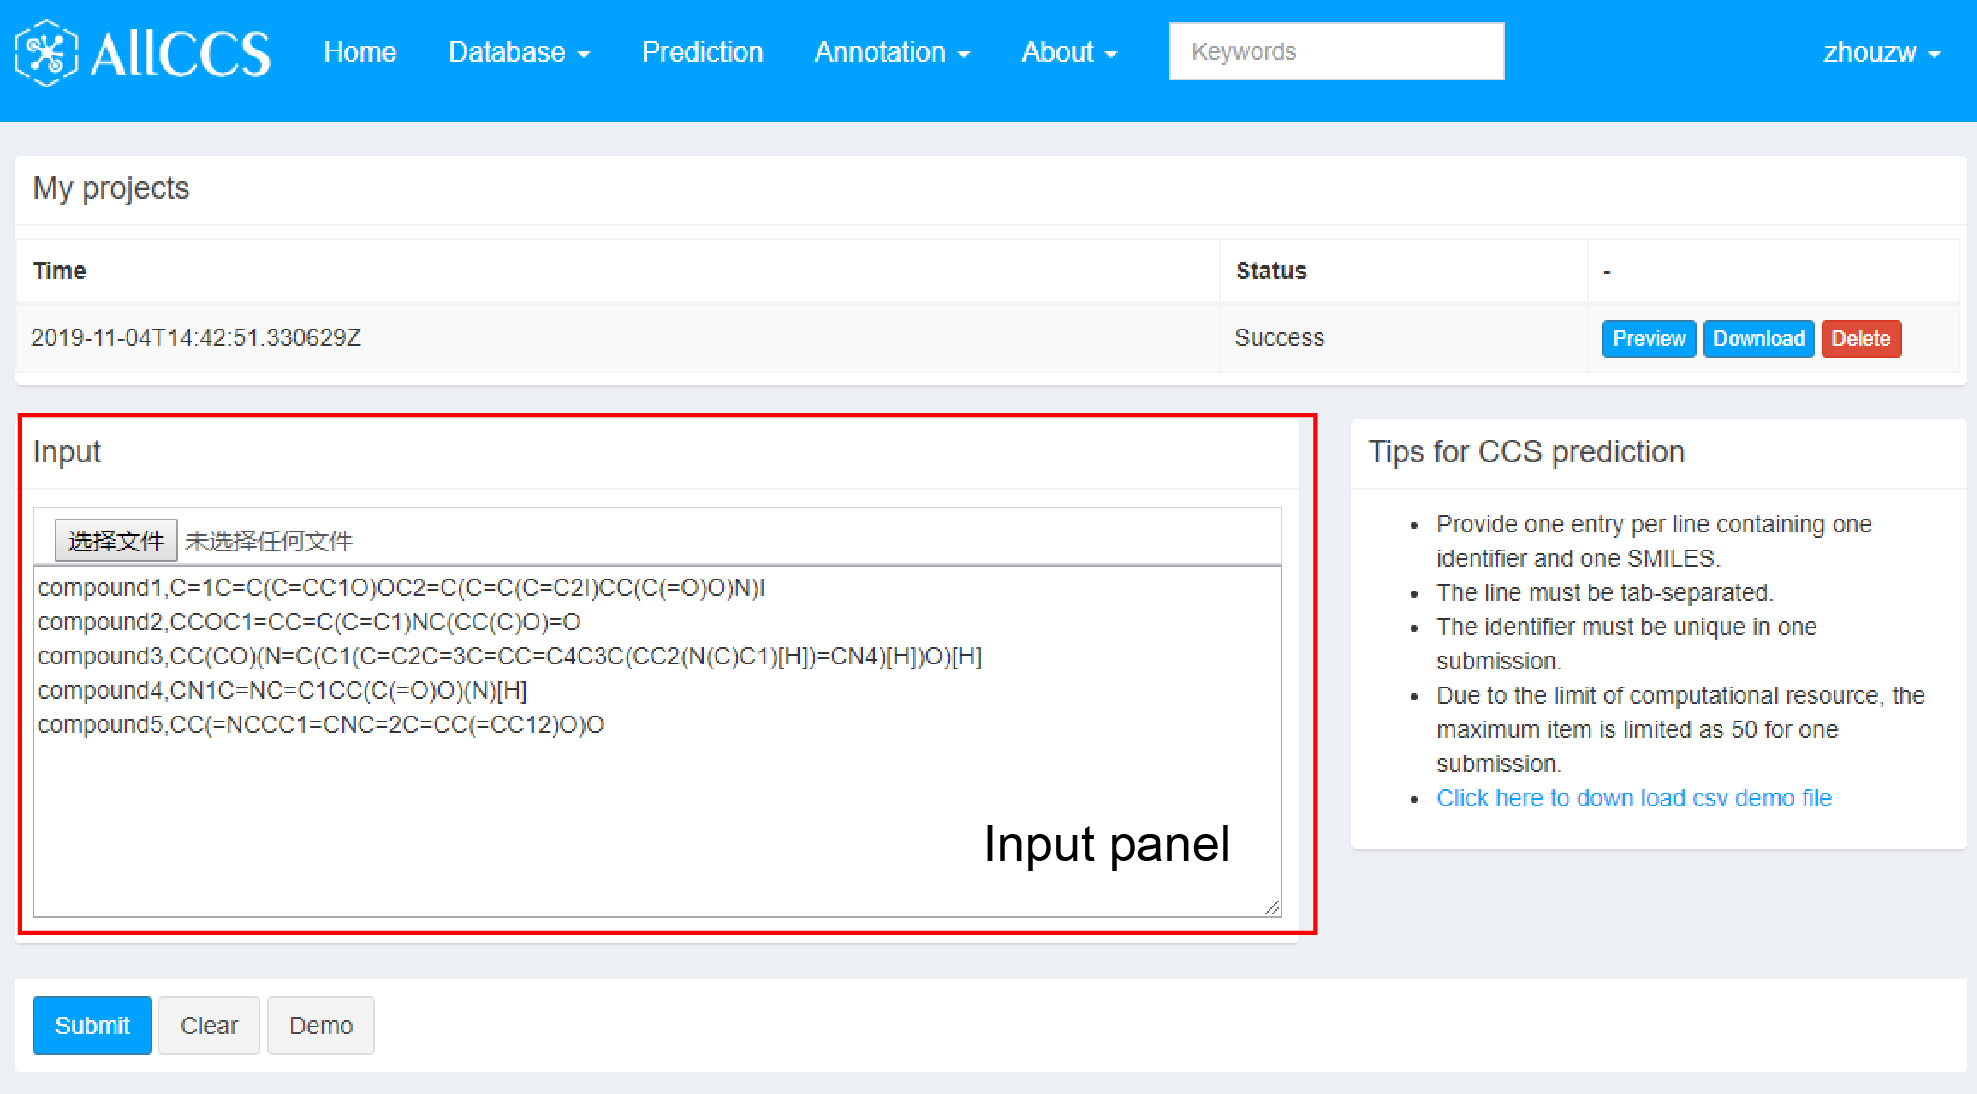
\includegraphics{images/chapter1/prediction} 

}

\caption{CCS prediction function}\label{fig:FigPrediction}
\end{figure}

For annotation function, you could search experimental feature to search
the database with your settings, or filter/rerank candidates to conjunct
with MS/MS annotation tools (Figure \ref{fig:FigMatch}).

\begin{figure}

{\centering 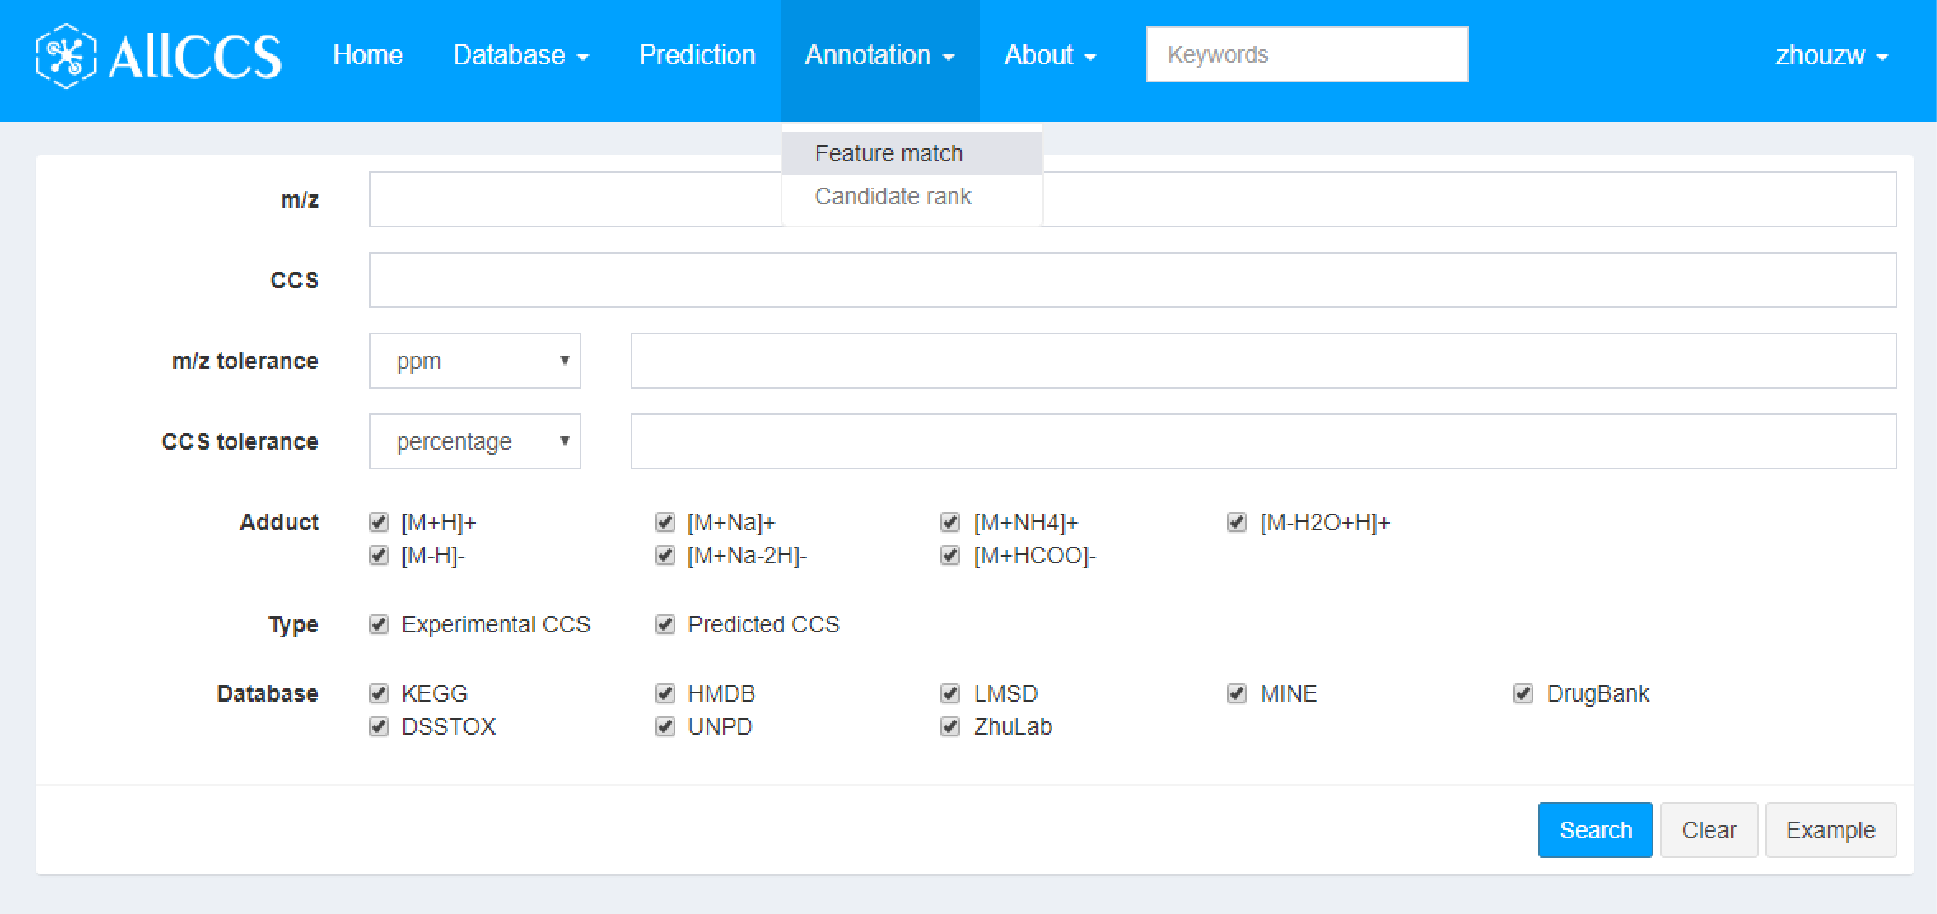
\includegraphics{images/chapter1/match} 

}

\caption{Metabolite match and candidate rank}\label{fig:FigMatch}
\end{figure}

\chapter{CCS Database}\label{chapter2}

Unified CCS database aims to be a \textbf{unified platform} to host both
literature-reported CCS values and in-silico predicted CCS values for
ion mobility - mass spectrometry (IM-MS). It is \textbf{open-access} and
\textbf{downloadable}. It contains 3,539 unified CCS values which are
summarized from 5,119 experimental CCS records. These experimental CCS
values are acquired with variable platform including DTIMS, TWIMS and
TIMS etc., and have definitive confidence level. In addition,
\textbf{\textasciitilde{}10,000,000 predicted CCS} values are provided
for \textbf{\textasciitilde{}1,700,000} small molecules from multiple
public database to support widespread applications, including
metabolomics, lipidomics, drug screening, pesticide screening etc (Table
\ref{tab:table2d1}). For each compound, its compound card contains meta
information, complete records and links to other database. Finally,
users can search interested compounds' CCS values with the function of
``Browser'' and/or ``Advance search'' in this part.

\begin{table}

\caption{\label{tab:table2d1}Basic statistics of Unified CCS database}
\centering
\begin{tabular}[t]{rlrlll}
\toprule
No. & Database & Compounds & Coverage & Mirror date & Reference\\
\midrule
1 & [KEGG](https://www.genome.jp/kegg/) & 16085 & Metabolites \& lipids & 2018-08-02 & @reference1\\
2 & [HMDB](http://www.hmdb.ca/) & 113989 & Metabolites \& lipids & 2018-06-09 & @reference2\\
3 & [LMSD](https://www.lipidmaps.org/) & 40532 & Metabolites \& lipids & 2019-07-11 & @reference3\\
4 & [MINE](https://minedatabase.mcs.anl.gov/) & 592175 & Metabolites \& lipids & 2018-02-07 & @reference4\\
5 & [DrugBank](https://www.drugbank.ca/) & 9546 & Drugs \& xenobiolics & 2019-04-12 & @reference5\\
\addlinespace
6 & [DSSTox](https://comptox.epa.gov/dashboard) & 856919 & Drugs \& xenobiolics & 2019-05-06 & @reference6\\
7 & [UNPD](NA) & 213188 & Natural products & 2019-06-13 & @reference7\\
8 & [ZhuLab](NA) & 1417 & Metabolites \& lipids & 2018-09-02 & @reference10\\
\bottomrule
\end{tabular}
\end{table}

\section{Compound Browser}\label{chapter2d1}

Compound Browser Function provides a simple and straightforward way to
browser the database. There are several browser conditions set in
``Browser'' part (Figure \ref{fig:figure2d1}).

\begin{itemize}
\tightlist
\item
  \textbf{Type}: It provides the choice of CCS values generated from
  experiments or prediction.
\item
  \textbf{Database}: this option includes variable databases that cover
  all compounds in our unified database (Table \ref{tab:table2d1}). And
  users can choose specific database(s) for further execution.
\item
  \textbf{Level}: it includes confidence level (See Section
  \ref{chapter2d2}) of compounds in the unified database. It helps to
  choose compounds in the clearly defined level.
\end{itemize}

\begin{figure}

{\centering 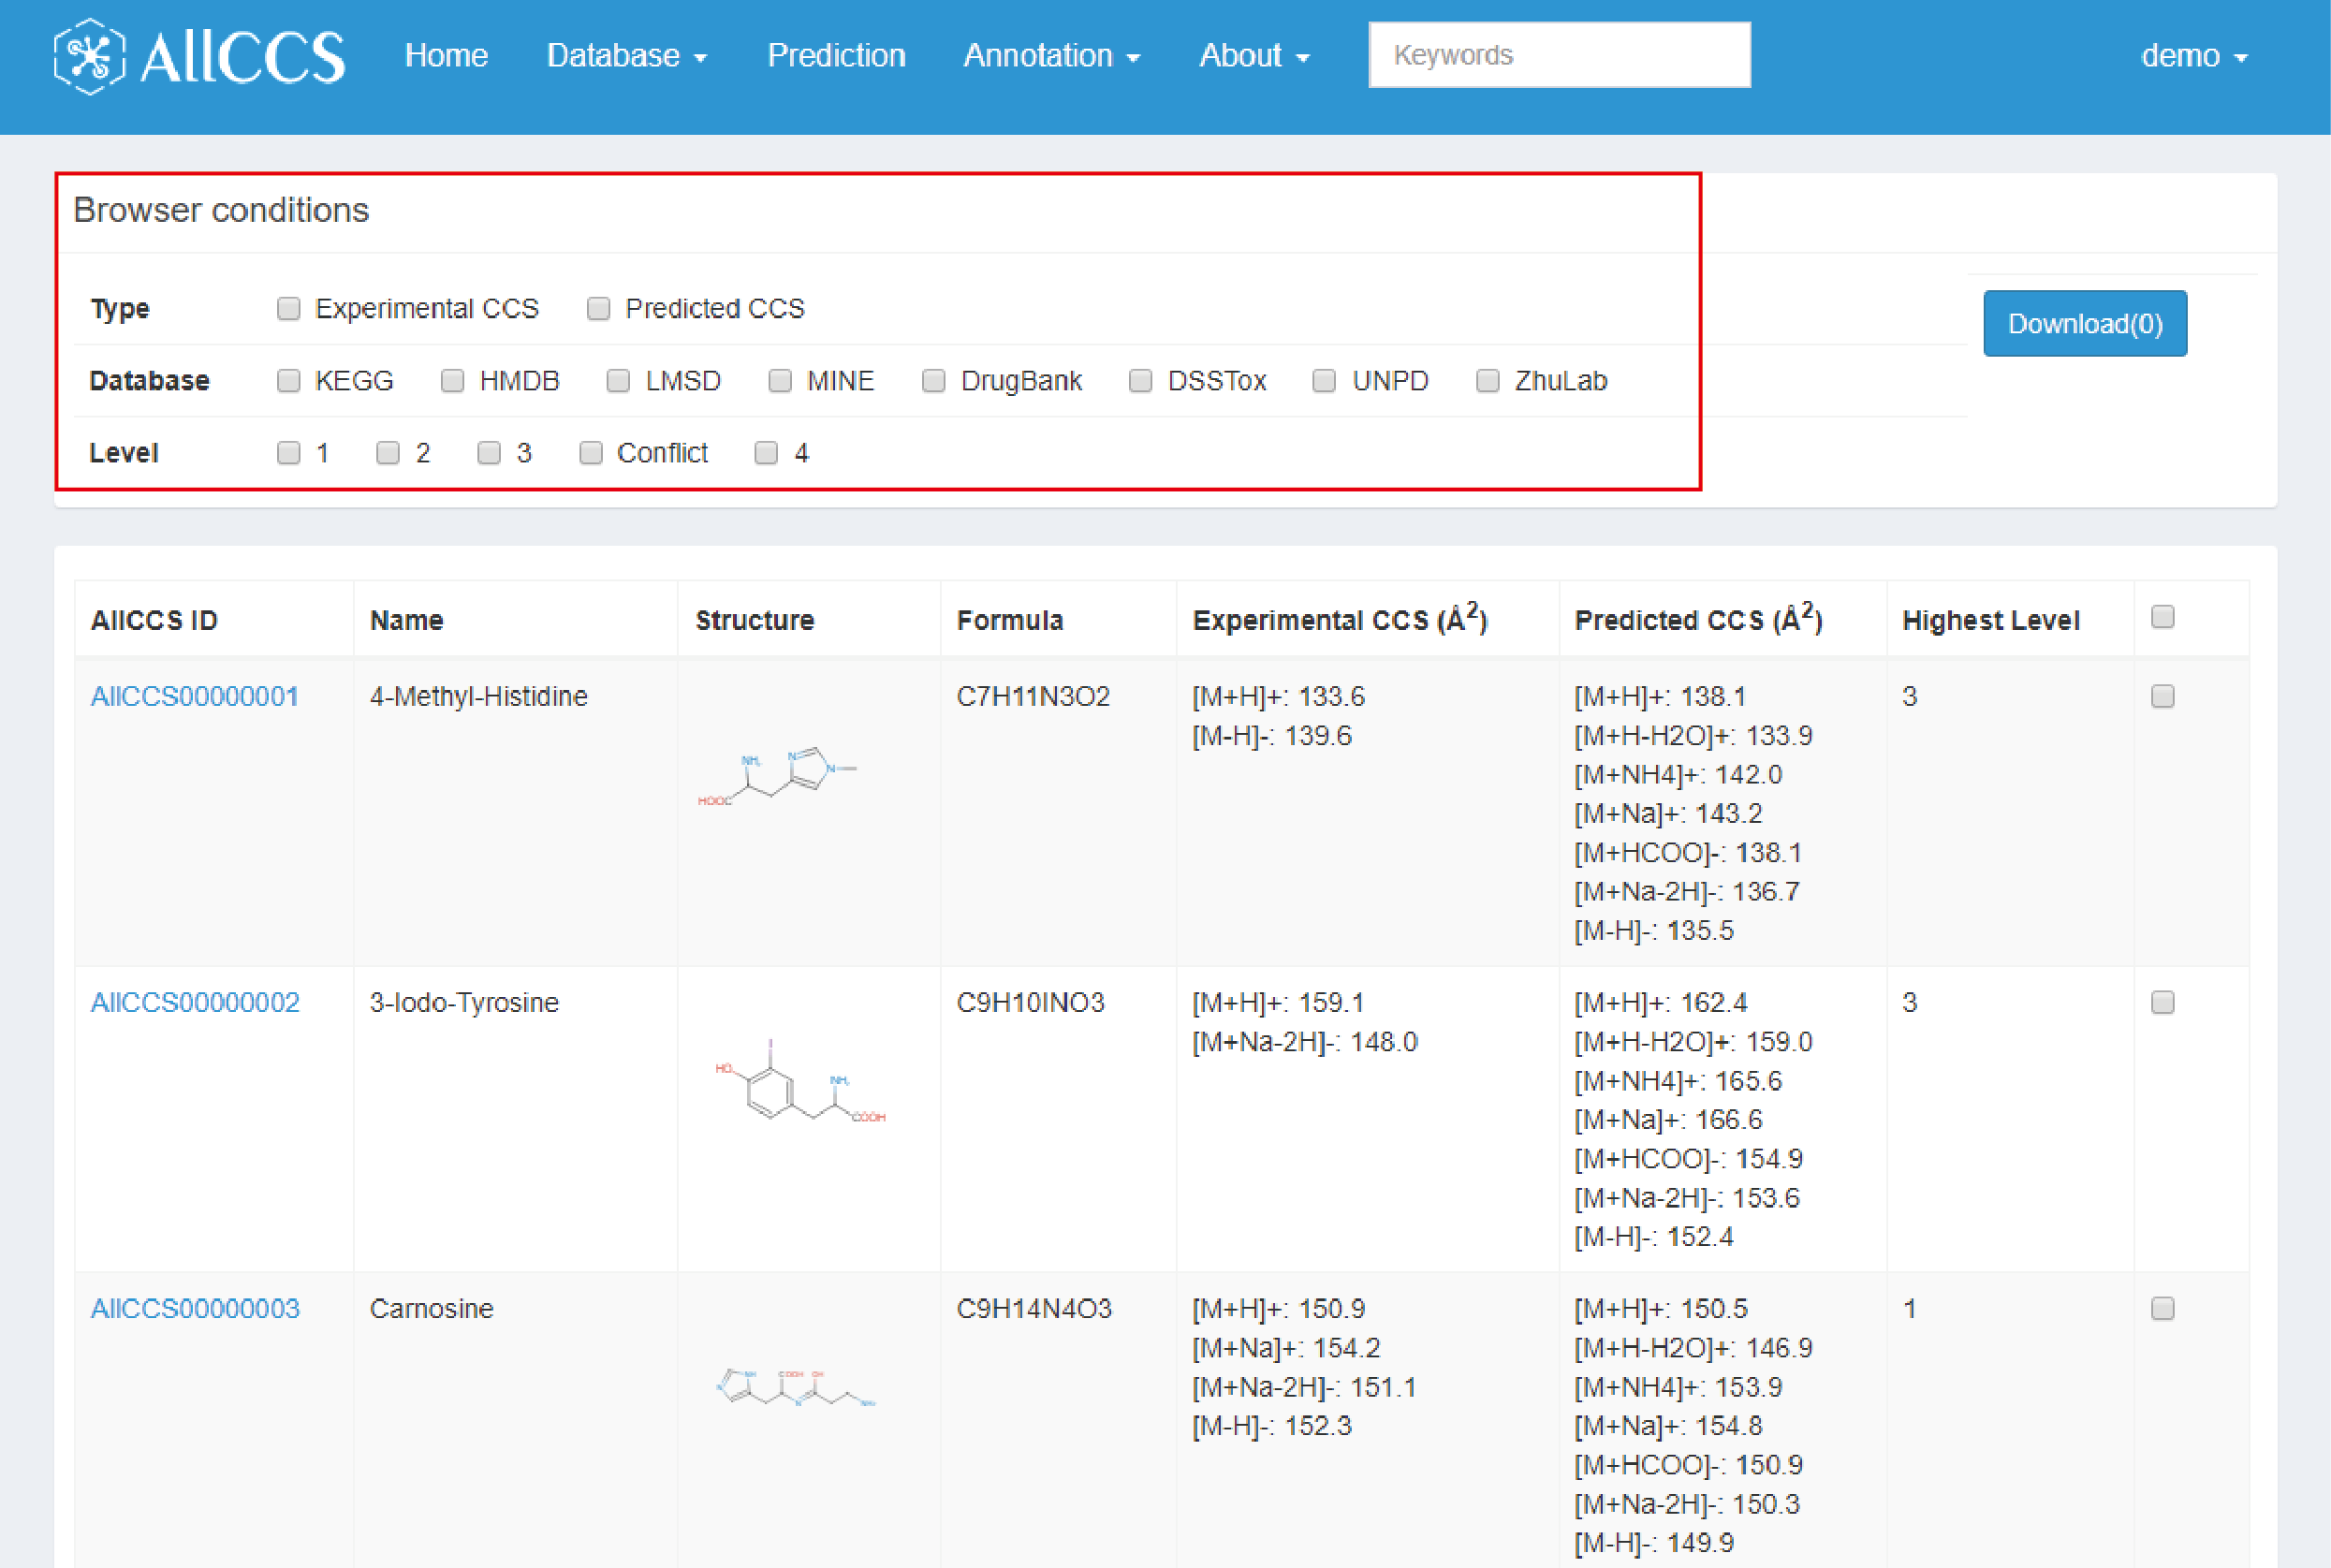
\includegraphics{images/chapter2/figure2.1browser_condition} 

}

\caption{Browser conditions}\label{fig:figure2d1}
\end{figure}

With browser conditions, users can screen out a series of interested
compounds. Compounds entries would be displayed according to defined
condition. In below text, it contains brief information for each
compound.

\begin{itemize}
\tightlist
\item
  \textbf{AllCCS ID}: As described in the section \ref{chaptere1d2},
  users can click the link in the column of AllCCS ID to browse the
  corresponding compound card (Figure \ref{fig:FigBrowser1}).
\item
  \textbf{Name}: compound name
\item
  \textbf{Structure}: the image of compound structure
\item
  \textbf{Formula}: chemical formula
\item
  \textbf{Experimental CCS}: The unified CCS value reported in
  literature (See Section \ref{chapter2d2d3})
\item
  \textbf{Predicted CCS}: The predicted CCS values using
  machine-learning algorithm. (See Section \ref{chapter2d2d4})
\item
  \textbf{Highest level}: The highest confidence level of CCS values
  (See Section \ref{chapter2d2d2})
\end{itemize}

Users can check the interested compounds in the last column. Click the
download option, you could download a CSV table containing the
information of you checked compounds (Figure \ref{fig:figure2d2}).

\textbf{Note}:

\begin{itemize}
\tightlist
\item
  Download function supports up to \textbf{100} items for one time.
\end{itemize}

\begin{figure}

{\centering 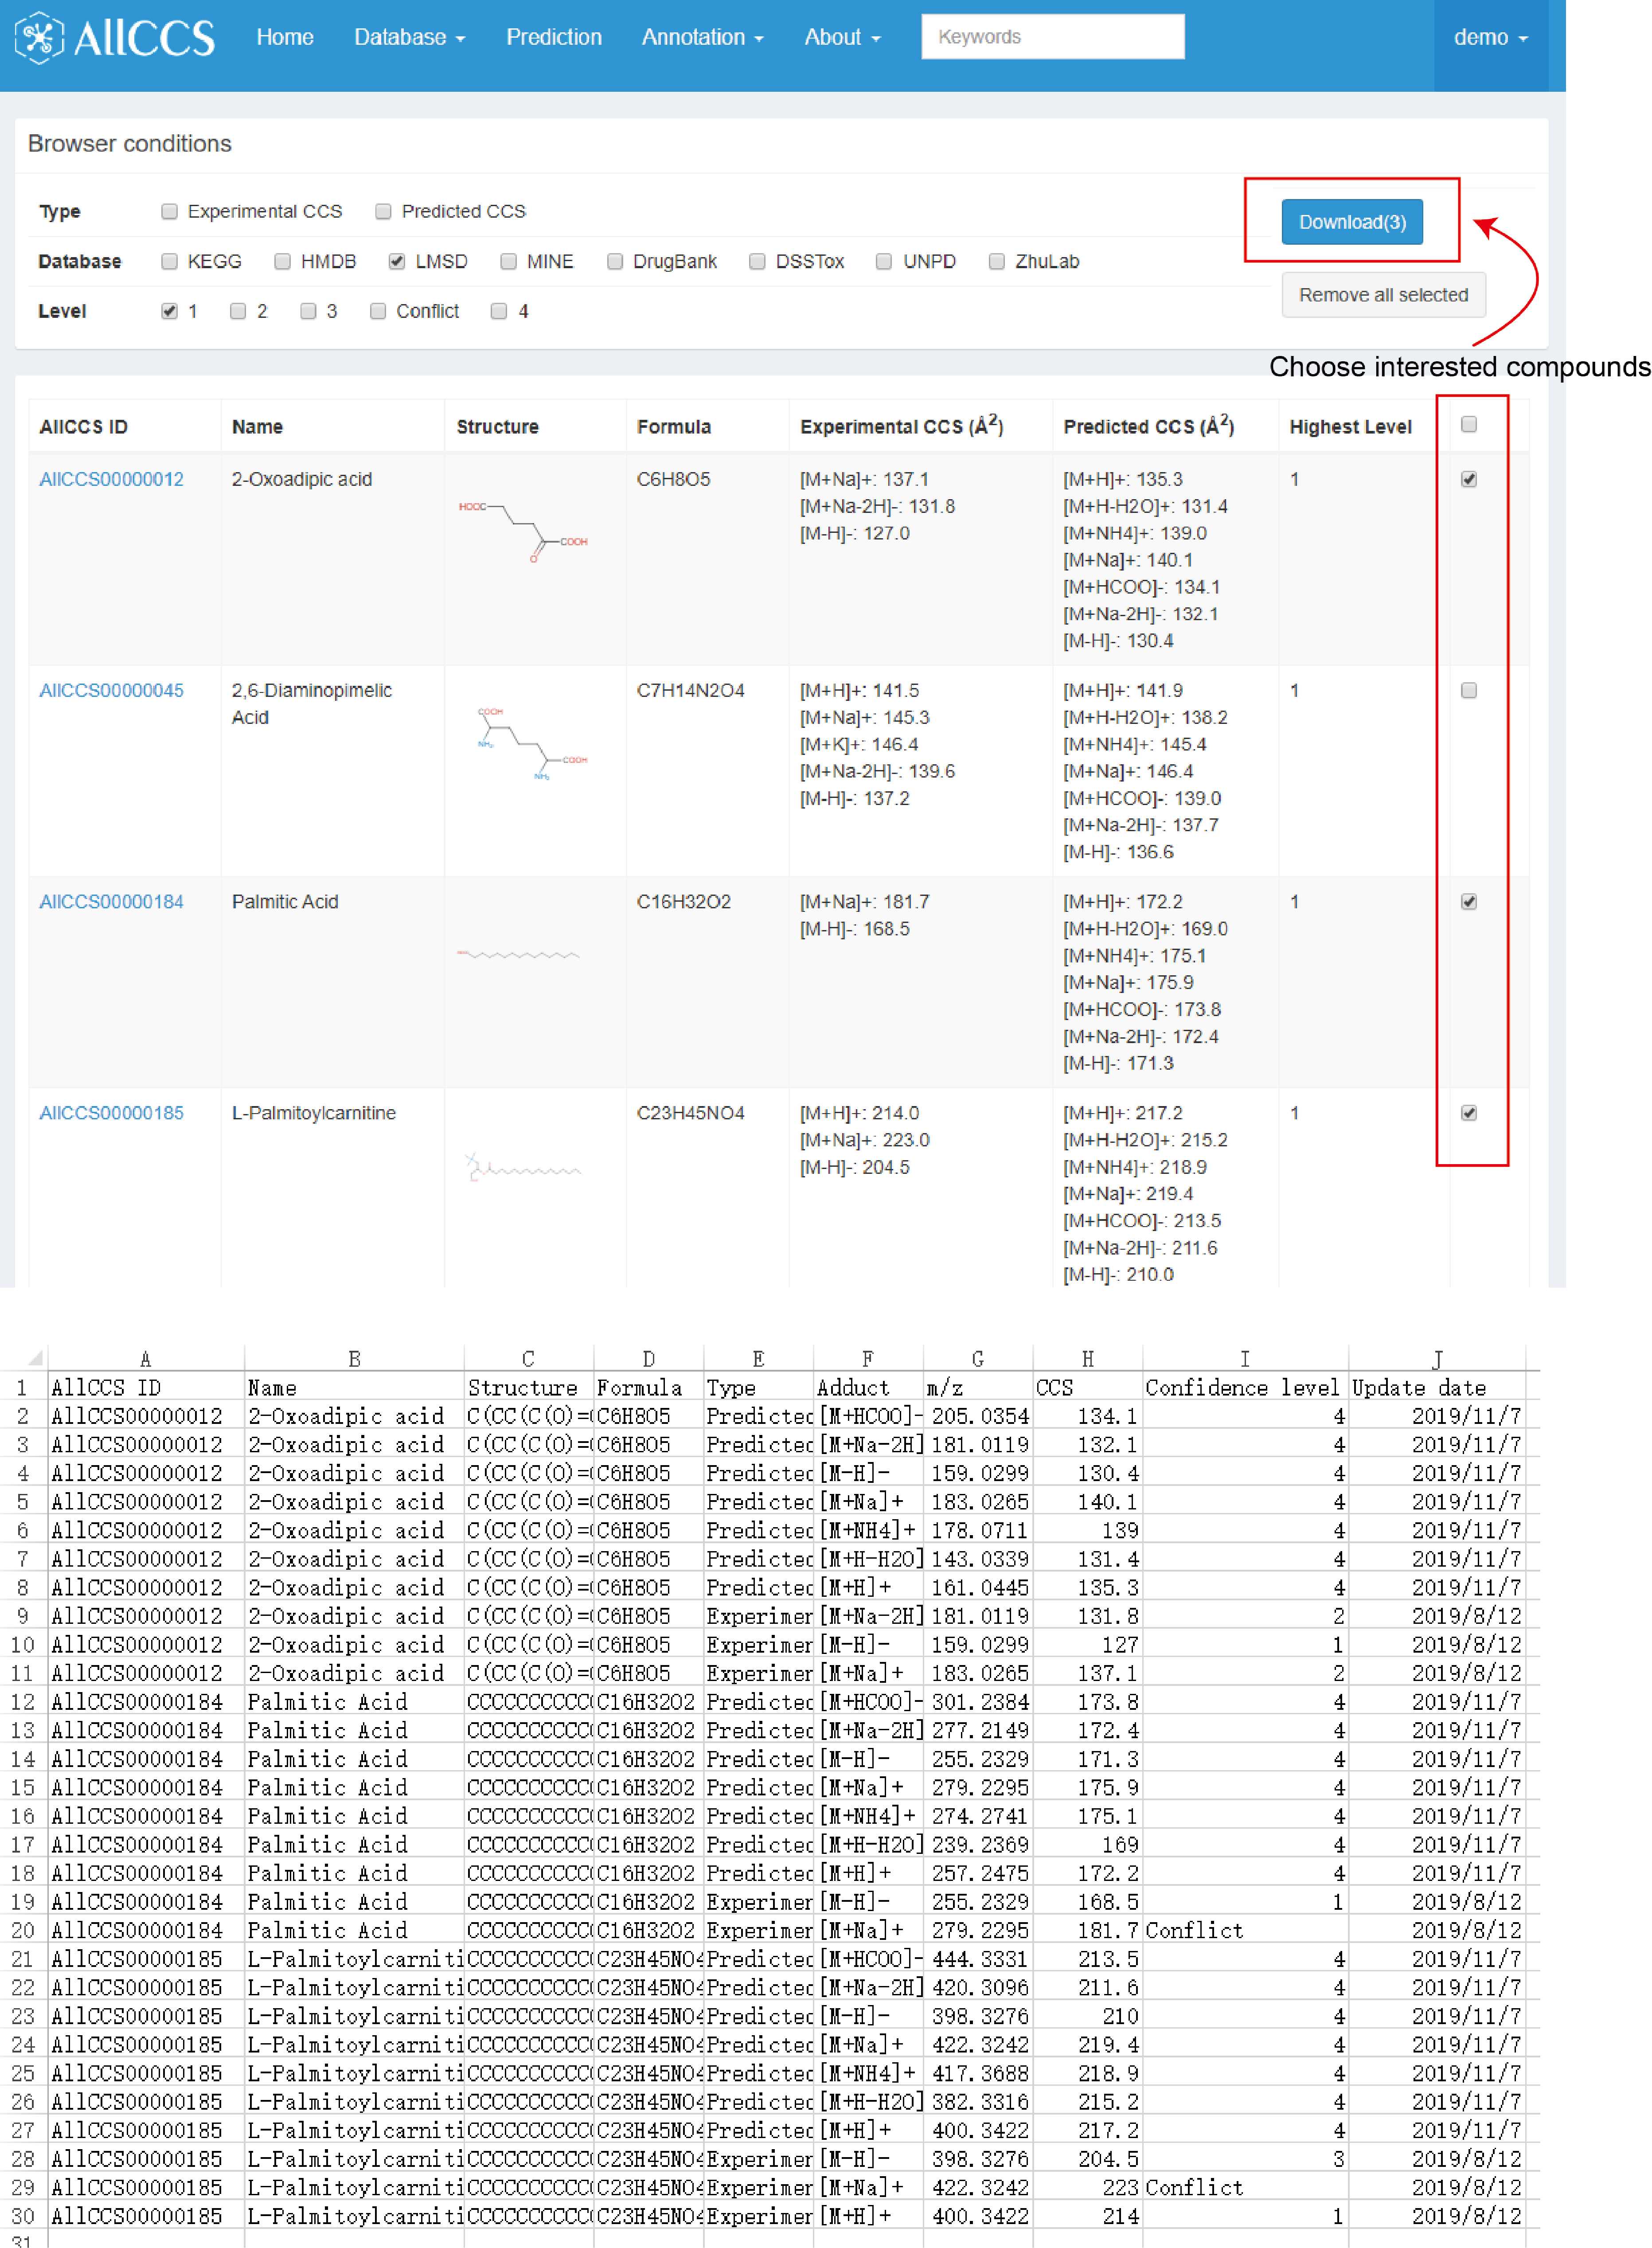
\includegraphics{images/chapter2/figure2.2browser_download_new} 

}

\caption{Download interested compounds}\label{fig:figure2d2}
\end{figure}

\section{Compound Card}\label{chapter2d2}

In the compound card, it contains detail information of the compound.
Next, we would like to explain each parts in the compound card.

\subsection{Compound information}\label{chapter2d2d1}

It contains the basic information of the compound, including ALLCCS ID,
name, formula, exact mass, SMILES, InChI, InChIKey, classification and
structure in the right panel (Figure \ref{fig:figure2d3}). Here,
\href{http://classyfire.wishartlab.com}{ClassyFire} is used for
compounds' classification \citep{reference8}.

\begin{figure}

{\centering 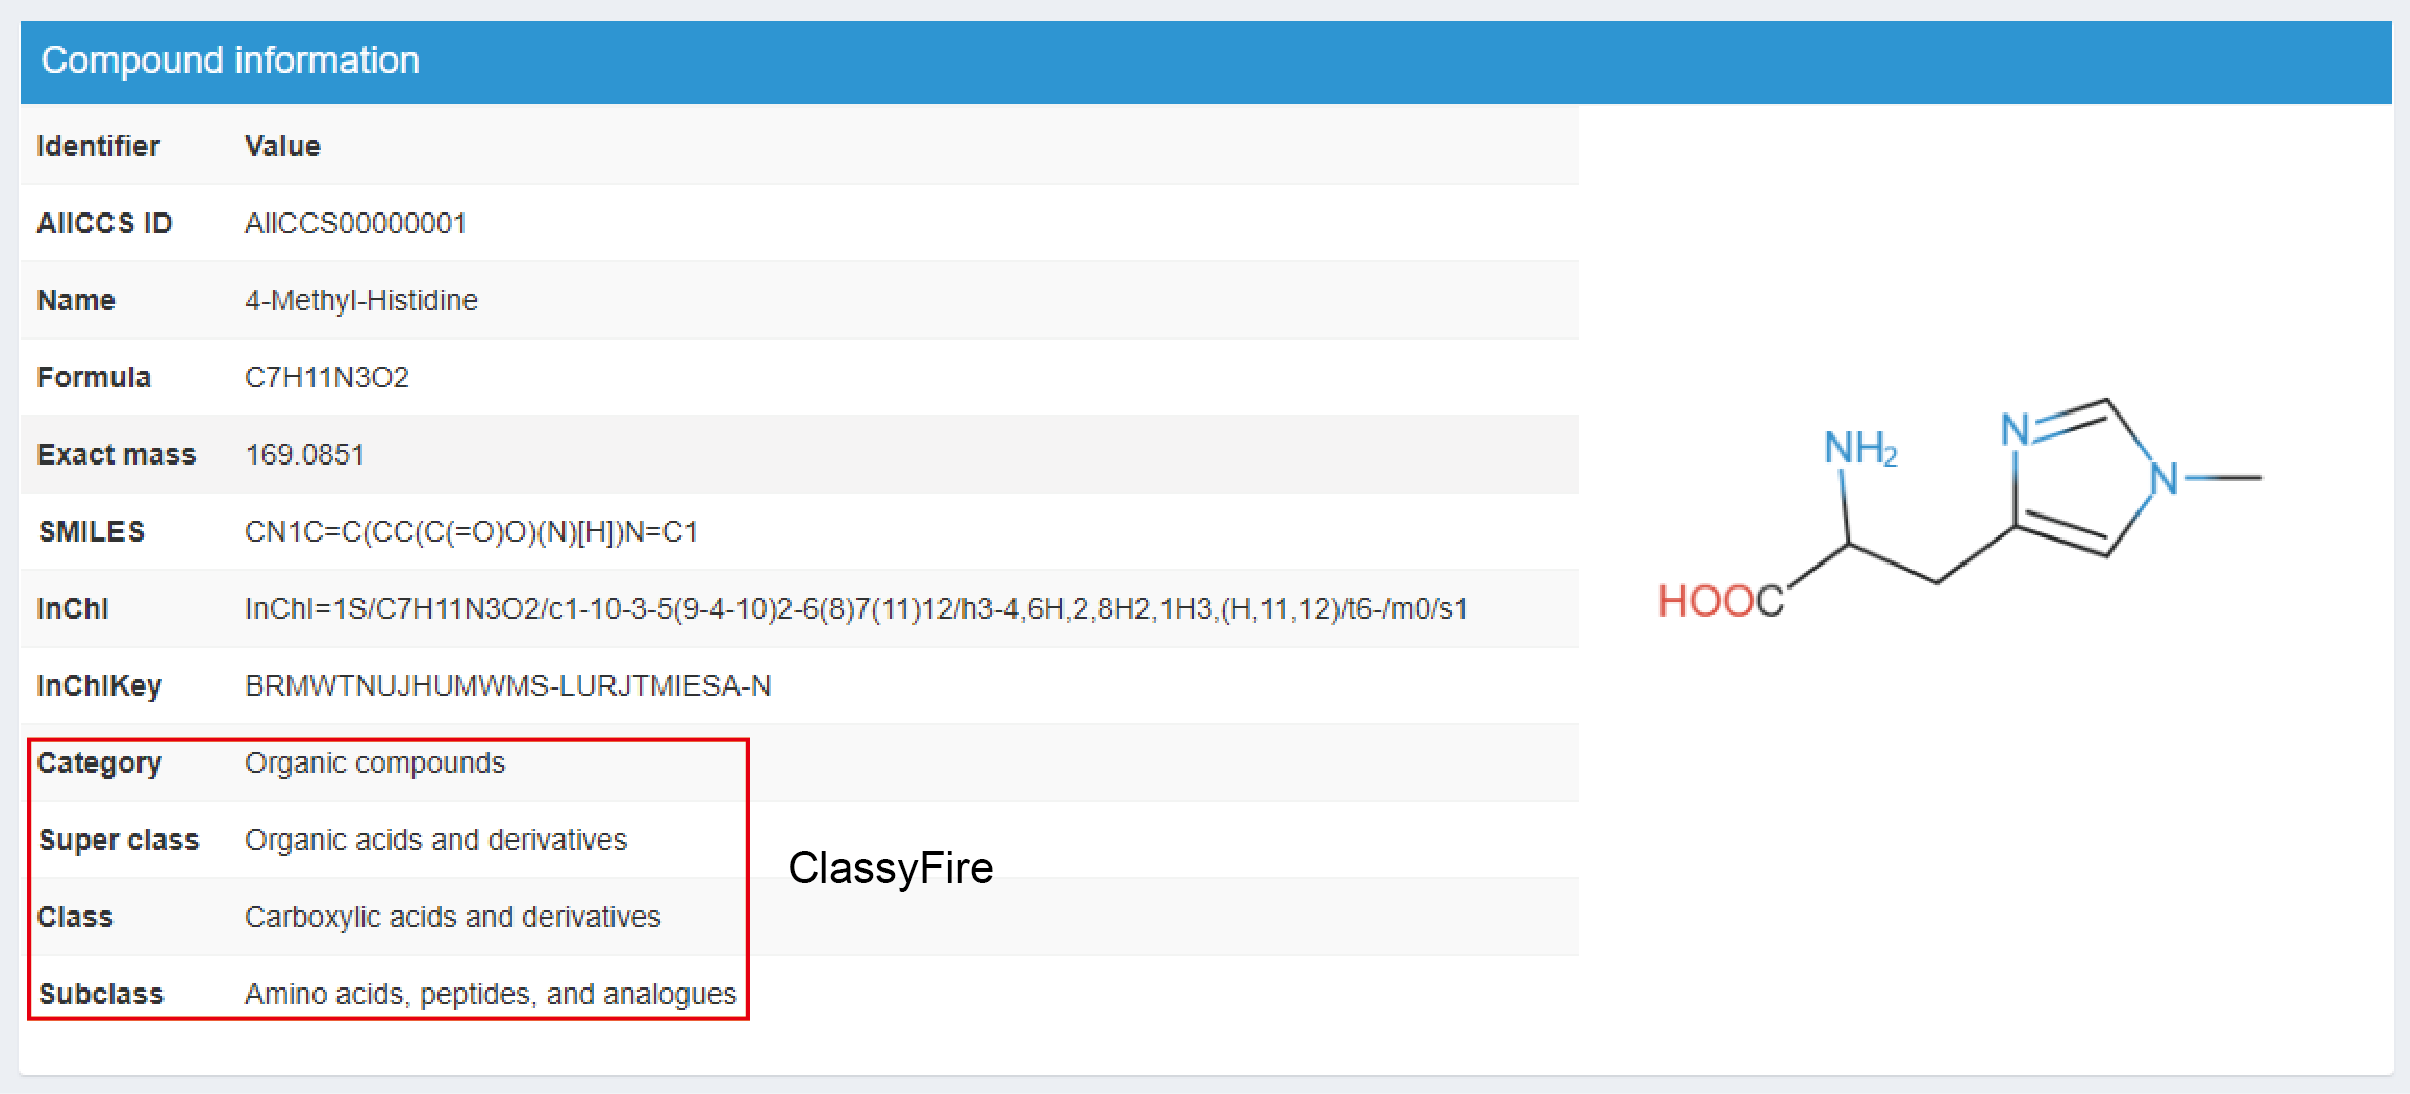
\includegraphics{images/chapter2/figure2.3compound_card_information} 

}

\caption{Download interested compounds}\label{fig:figure2d3}
\end{figure}

\subsection{Unified CCS}\label{chapter2d2d2}

This part contains the CCS information of different adduct forms with
experimental CCS (if exists) and predicted CCS (Figure
\ref{fig:figure2d4}). The CCS reported here is the unified CCS values.
We defined unified CCS as the average CCS value with definitive
confidence level. The definition of confidence level can find in Table
\ref{tab:table2d2}. CCS values of confidence 1, 2, 3 are all
experimental values. The definition of confidence level:

\begin{table}

\caption{\label{tab:table2d2}Definition of confidence level}
\centering
\begin{tabular}[t]{llll}
\toprule
Confidence level & Platform & Reported labs (N) & Maximum relative error (\%)\\
\midrule
Level 1 & DTIMS & N≥2 & ≤1\%\\
Level 2 & DTIMS/TWIMS/TIMS & N≥2 & ≤3\%\\
Level 3 & DTIMS/TWIMS/TIMS & N=1 & ---\\
Level 4 & Predicted CCS & --- & ---\\
Conflict & DTIMS/TWIMS/TIMS & N≥2 & >3\%\\
\bottomrule
\end{tabular}
\end{table}

\begin{itemize}
\tightlist
\item
  \textbf{Confidence level 1} represents the CCS value of the specie
  which is acquired with DTIMS and has been reported at least twice in
  different labs with the maximum relative error less than 1\%.
\item
  \textbf{Confidence level 2} represents the CCS value of specie which
  is acquired with DTIMS, TWIMS or TIMS and has been reported at least
  twice in different labs with the maximum relative error less than 3\%.
\item
  \textbf{Confidence level 3} represents the CCS value of specie is
  acquired with DTIMS, TWIMS or TIMS and only reported by one lab.
\item
  \textbf{Confidence level 4} represents the predicted CCS value.
\item
  \textbf{Conflict} means the CCS value of specie which is acquired with
  DTIMS, TWIMS or TIMS and has been reported at least twice in different
  labs, but the maximum relative error is more than 3\%.
\end{itemize}

\begin{figure}

{\centering 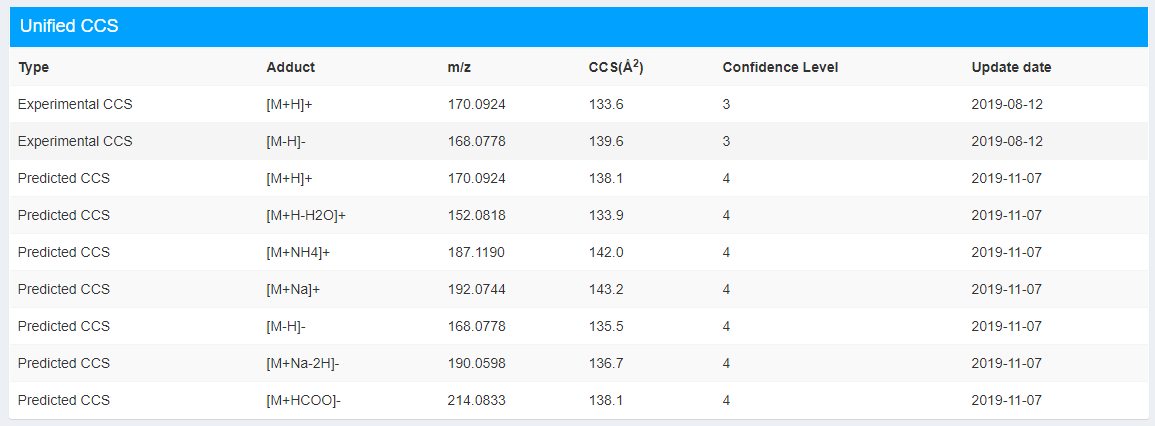
\includegraphics{images/chapter2/figure2.4unified_ccs} 

}

\caption{Unified CCS}\label{fig:figure2d4}
\end{figure}

\subsection{Experimental CCS records}\label{chapter2d2d3}

This part records the detailed information of experimental CCS values
(Figure \ref{fig:figure2d5}). Compounds that have experimental CCS
records contains the basic information of adduct form, m/z, experimental
CCS values and charge. Besides, we also provide the information of used
instrument platform and the type of ion mobility mass spectrometry.
Detail information can be found in Table \ref{tab:table2d3}. The
measured approach is also provided, including single-field,
multiple-fields, and empirical method. Corresponding reference
literature is listed in the DOI column. If compounds don't have
experimental CCS record, it would have no information in this part.

\begin{table}

\caption{\label{tab:table2d3}IM-MS Instruments in AllCCS}
\centering
\begin{tabular}[t]{lll}
\toprule
Instrument & Type & Vendor\\
\midrule
Agilent 6560 DTIM-QTOF & DTIMS & Agilent\\
Waters Synapt G2-Si HDMS & TWIMS & Waters\\
Waters Synapt G2 HDMS & TWIMS & Waters\\
Waters Vion IMS QTOF & TWIMS & Waters\\
TOFwerk IMS TOF & DTIMS & TOFwerk\\
\addlinespace
Bruker timsTOF & TIMS & Bruker\\
Bruker timsTOF Pro & TIMS & Bruker\\
\bottomrule
\end{tabular}
\end{table}

\begin{figure}

{\centering 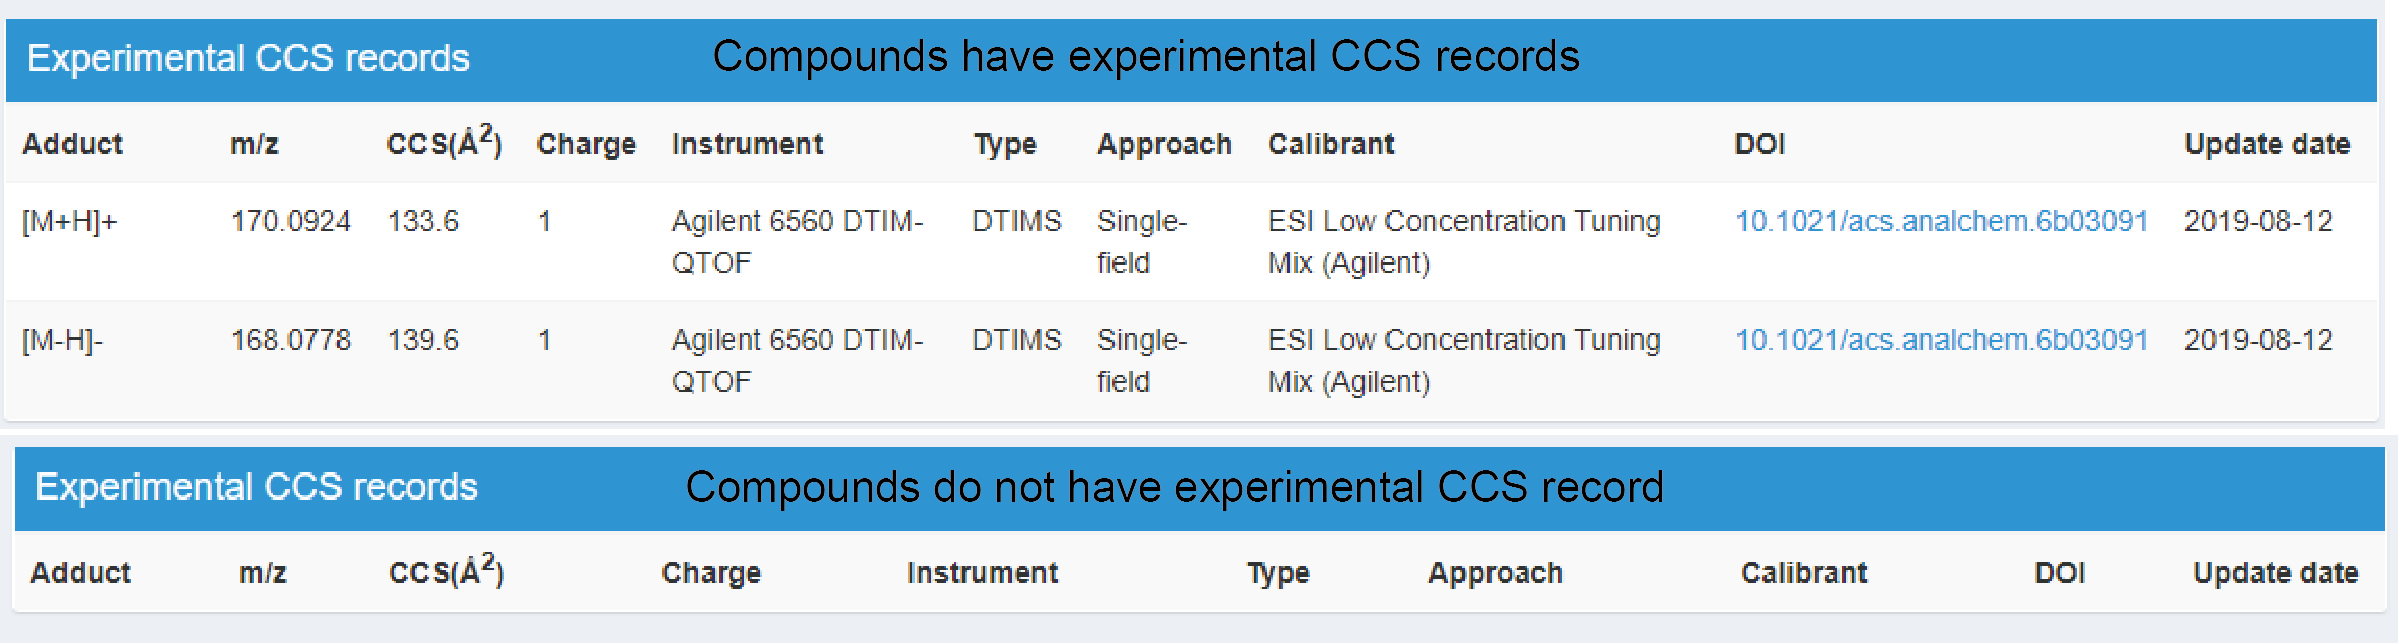
\includegraphics{images/chapter2/figure2.5compound_card_exp_ccs} 

}

\caption{Experimental CCS records}\label{fig:figure2d5}
\end{figure}

\subsection{Predicted CCS records}\label{chapter2d2d4}

This part records the detailed information of predicted CCS values
(Figure \ref{fig:figure2d6}). It provides the basic information of
adduct forms, m/z, charge, corresponding predicted CCS values using
AllCCS\_V1 tool, users can reference AllCCS paper for detailed
information \citep{reference10}. Here we define representative structure
similarity (RSS) to represent the similarity between this compound and
the training set.

\begin{figure}

{\centering 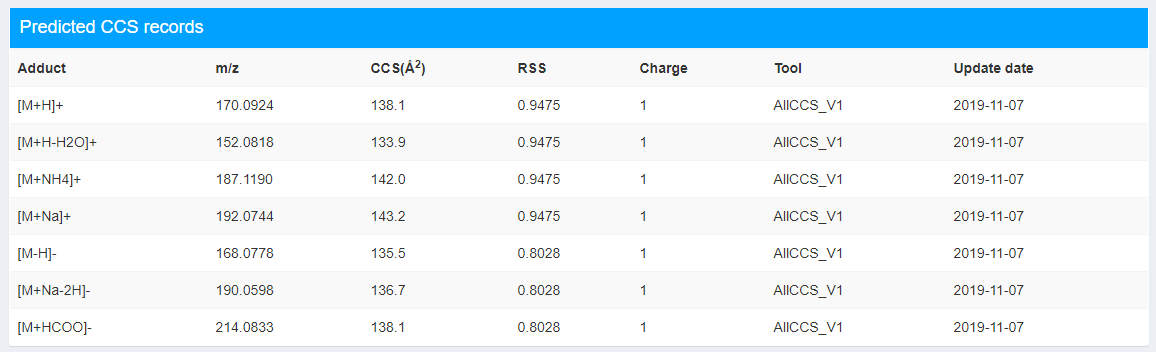
\includegraphics{images/chapter2/figure2.6predicted_ccs} 

}

\caption{Predicted CCS records}\label{fig:figure2d6}
\end{figure}

\subsection{Database link}\label{chapter2d2d5}

This part provides the link to databases that contain the compound
(Figure \ref{fig:figure2d7}).

\begin{figure}

{\centering 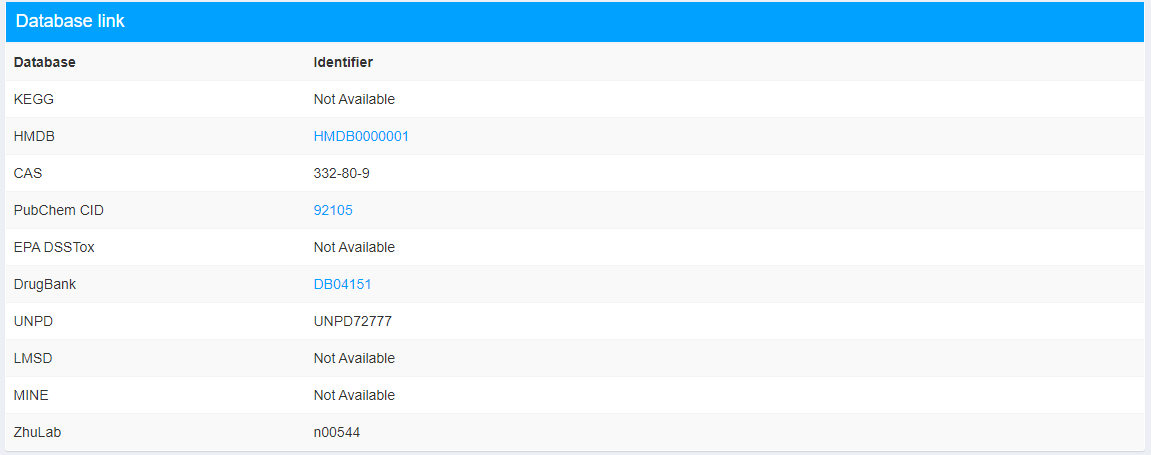
\includegraphics{images/chapter2/figure2.7database_link} 

}

\caption{Database link}\label{fig:figure2d7}
\end{figure}

\section{Advanced Search}\label{chapter2d3}

For advanced search, there are two modes for users to search the
compounds in our unified CCS database, including \textbf{``single
mode''} and \textbf{``batch mode''}.

\subsection{Single mode}\label{chapter2d3d1}

As named, users can search for one compounds at one time in single mode.
Here, we provide several optional identifiers for users to choose
(Figure \ref{fig:figure2d8}), including compound's name, database ID,
formula, SMILES, InChI, InChIKey.

\textbf{Note}:

\begin{itemize}
\tightlist
\item
  If you don't have confirmed identifier, keep it as null.
\item
  If there are contradictory identifier, it will return no available
  data.
\end{itemize}

\begin{figure}

{\centering 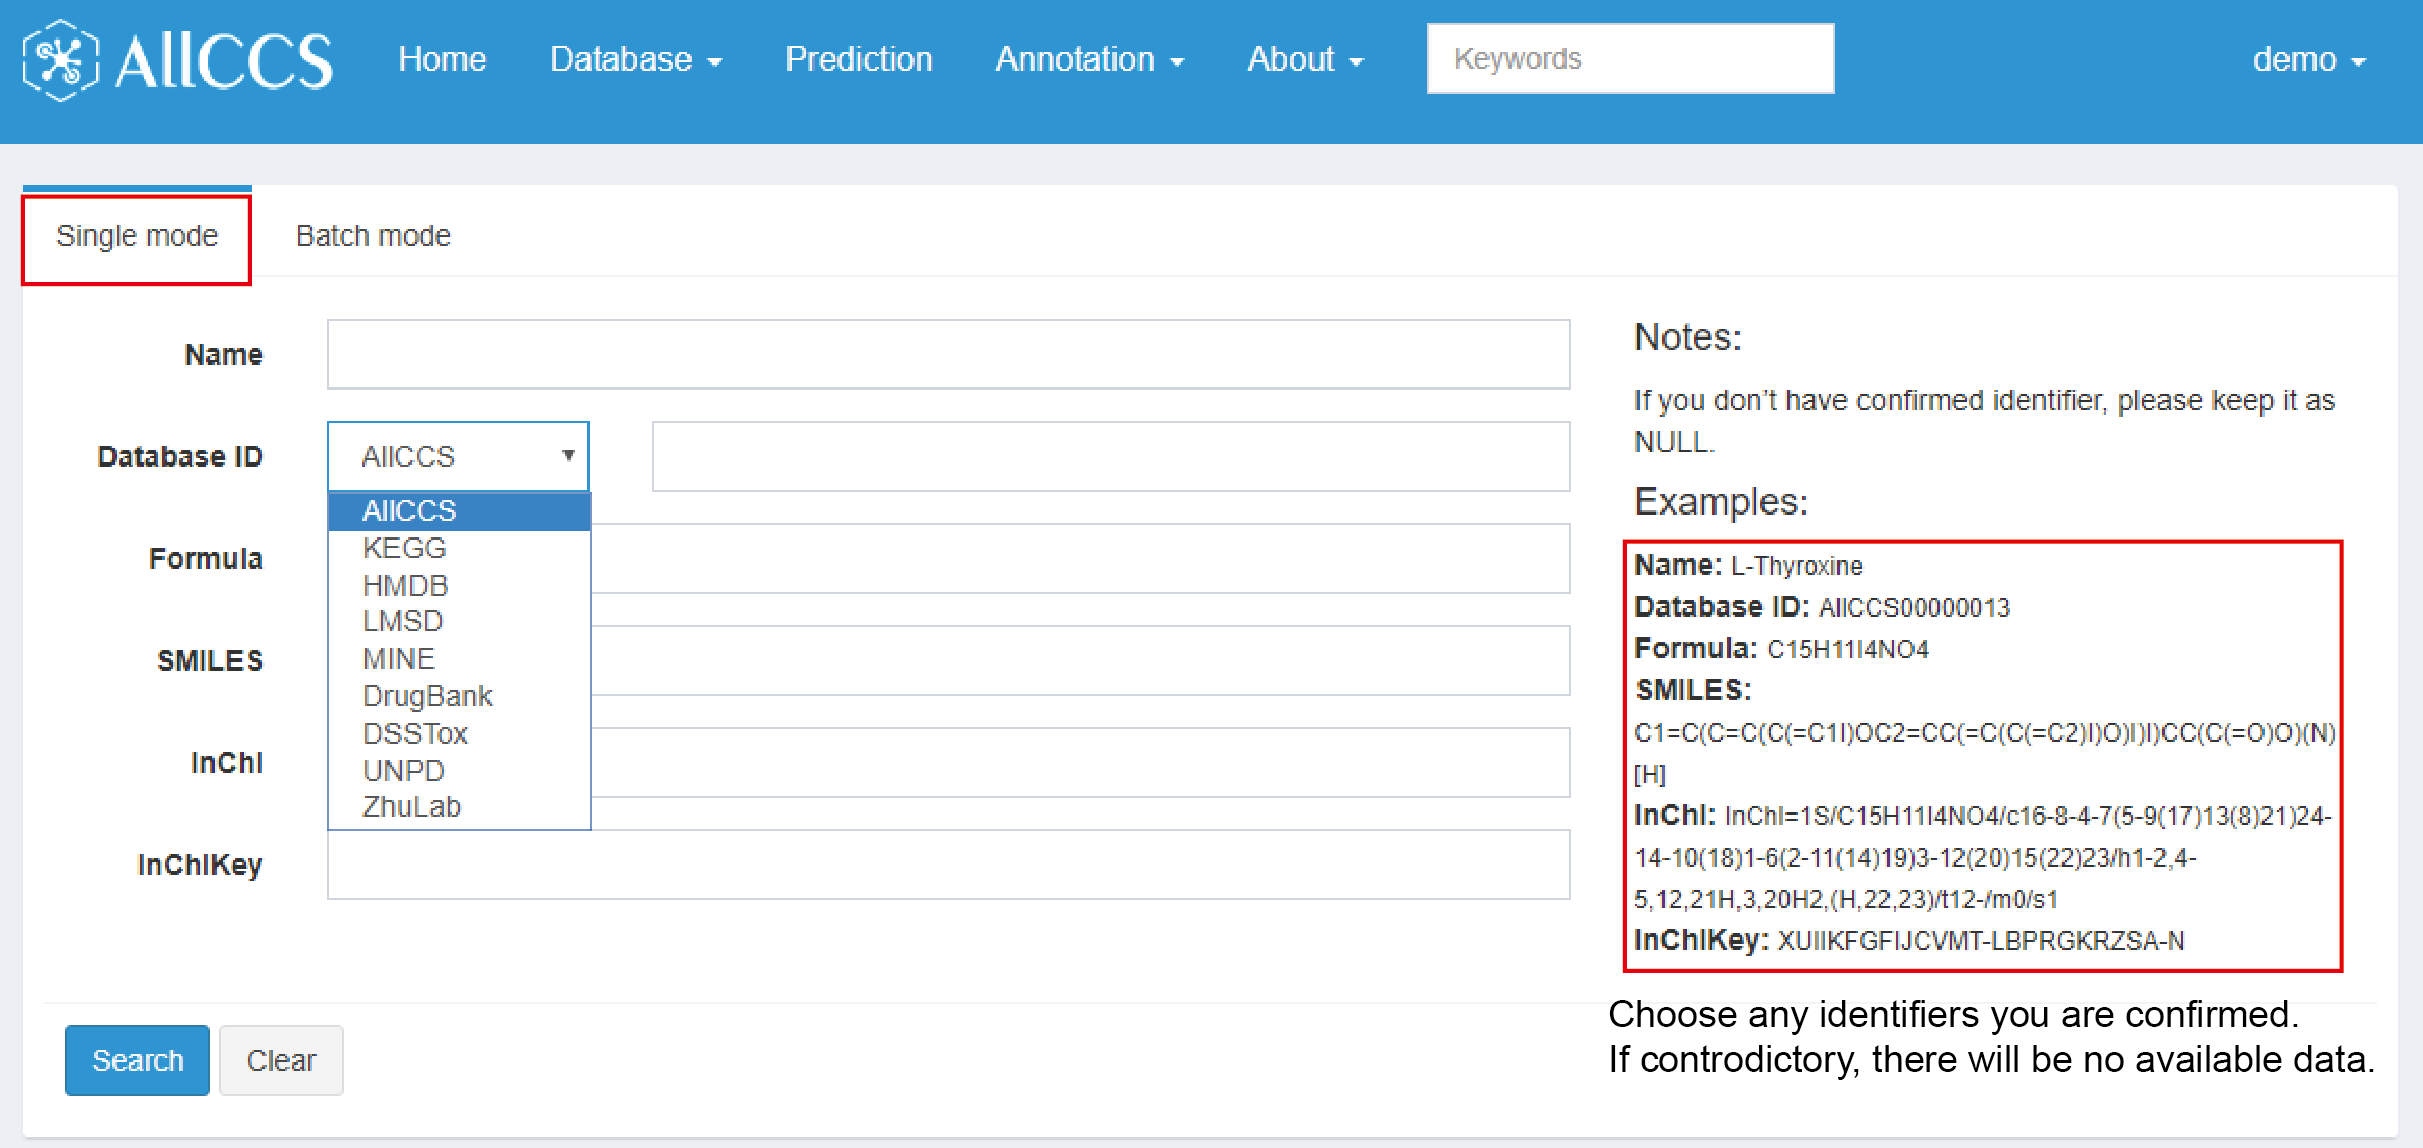
\includegraphics{images/chapter2/figure2.8advance_search_single} 

}

\caption{Advanced search – single mode}\label{fig:figure2d8}
\end{figure}

\subsection{Batch mode}\label{chapter2d3d2}

If there are multiple compounds, users can use batch mode to search
(Figure \ref{fig:figure2d9}). Currently, this function supports
identifiers including ``Database ID'', SMILES, InChIKey. While choosing
database ID as identifier, there are several choice of databases in the
right panel close to identifier option.

\textbf{Note}:

\begin{itemize}
\tightlist
\item
  In searching panel, you can enter one item per line.
\item
  It should not contain extra space.
\item
  It supports up to 100 query items per request.
\end{itemize}

\begin{figure}

{\centering 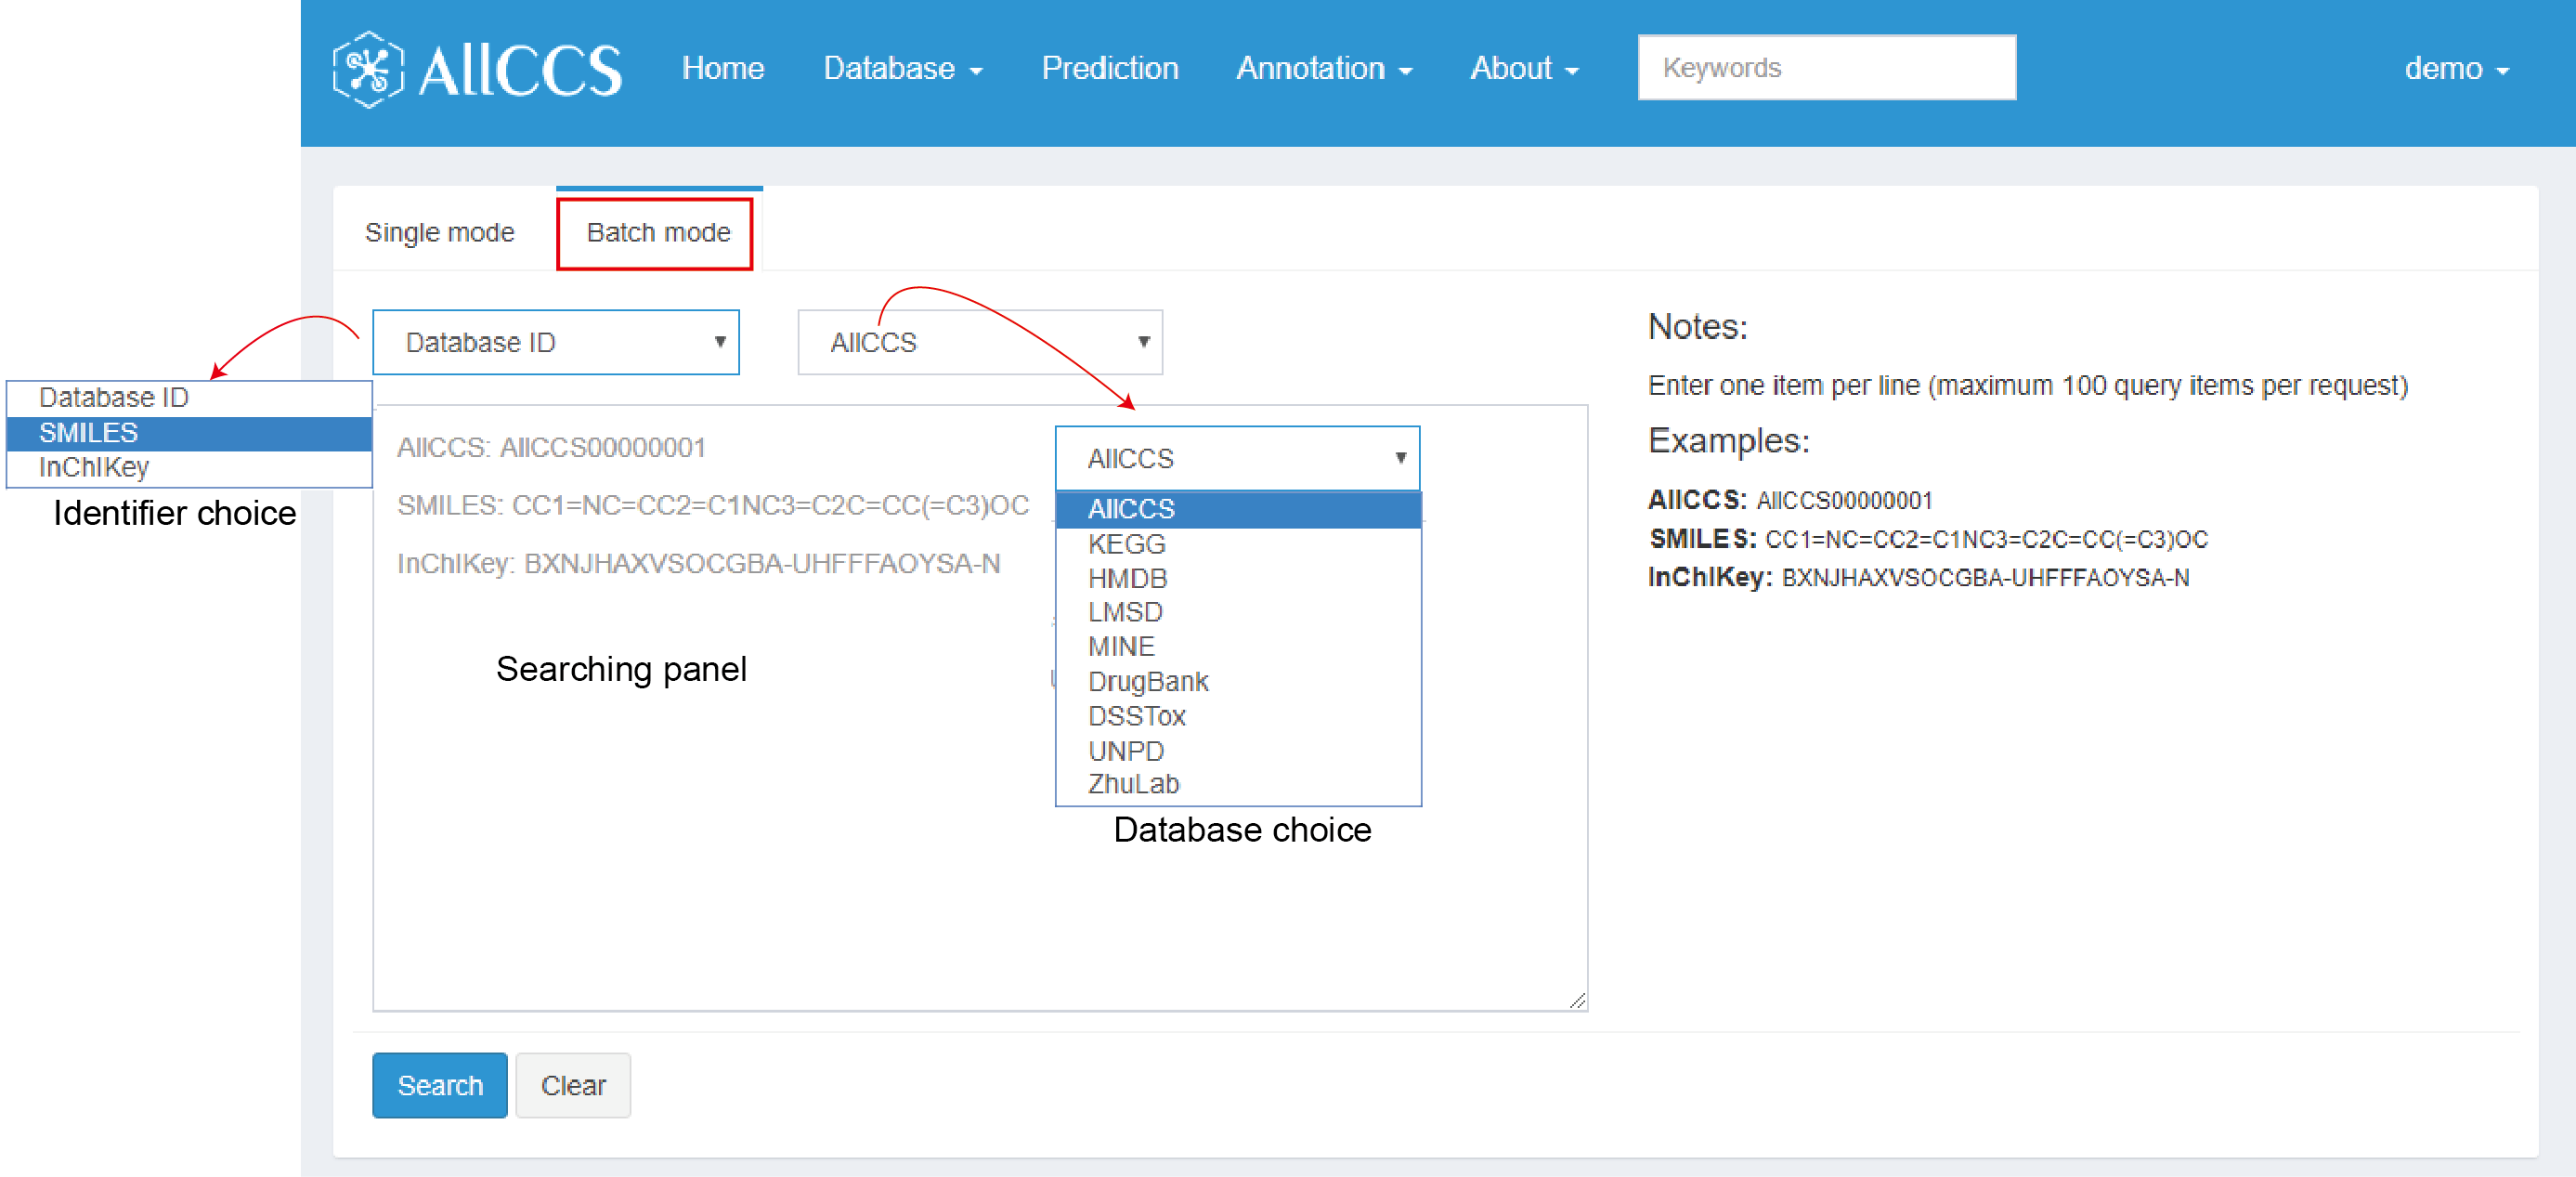
\includegraphics{images/chapter2/figure2.9advance_search_batch} 

}

\caption{Advanced search – batch mode}\label{fig:figure2d9}
\end{figure}

\chapter{CCS Prediction}\label{chapter3}

This part provides a machine-learning based CCS prediction function with
the input of SMILES structures. The prediction error is estimated as low
as \textasciitilde{}2\% (Median relative error), and users could predict
CCS values for novel structures. Detail of prediction is provided in our
AllCCS article \textbf{【ref10】}.

\section{Data preparation}\label{chapter3d1}

For CCS prediction, users should provide the SMILES and the unique
identifier for each SMILES. And there are two approaches for users to
search in the interface (Figure \ref{fig:figure3d1}).

\begin{figure}

{\centering 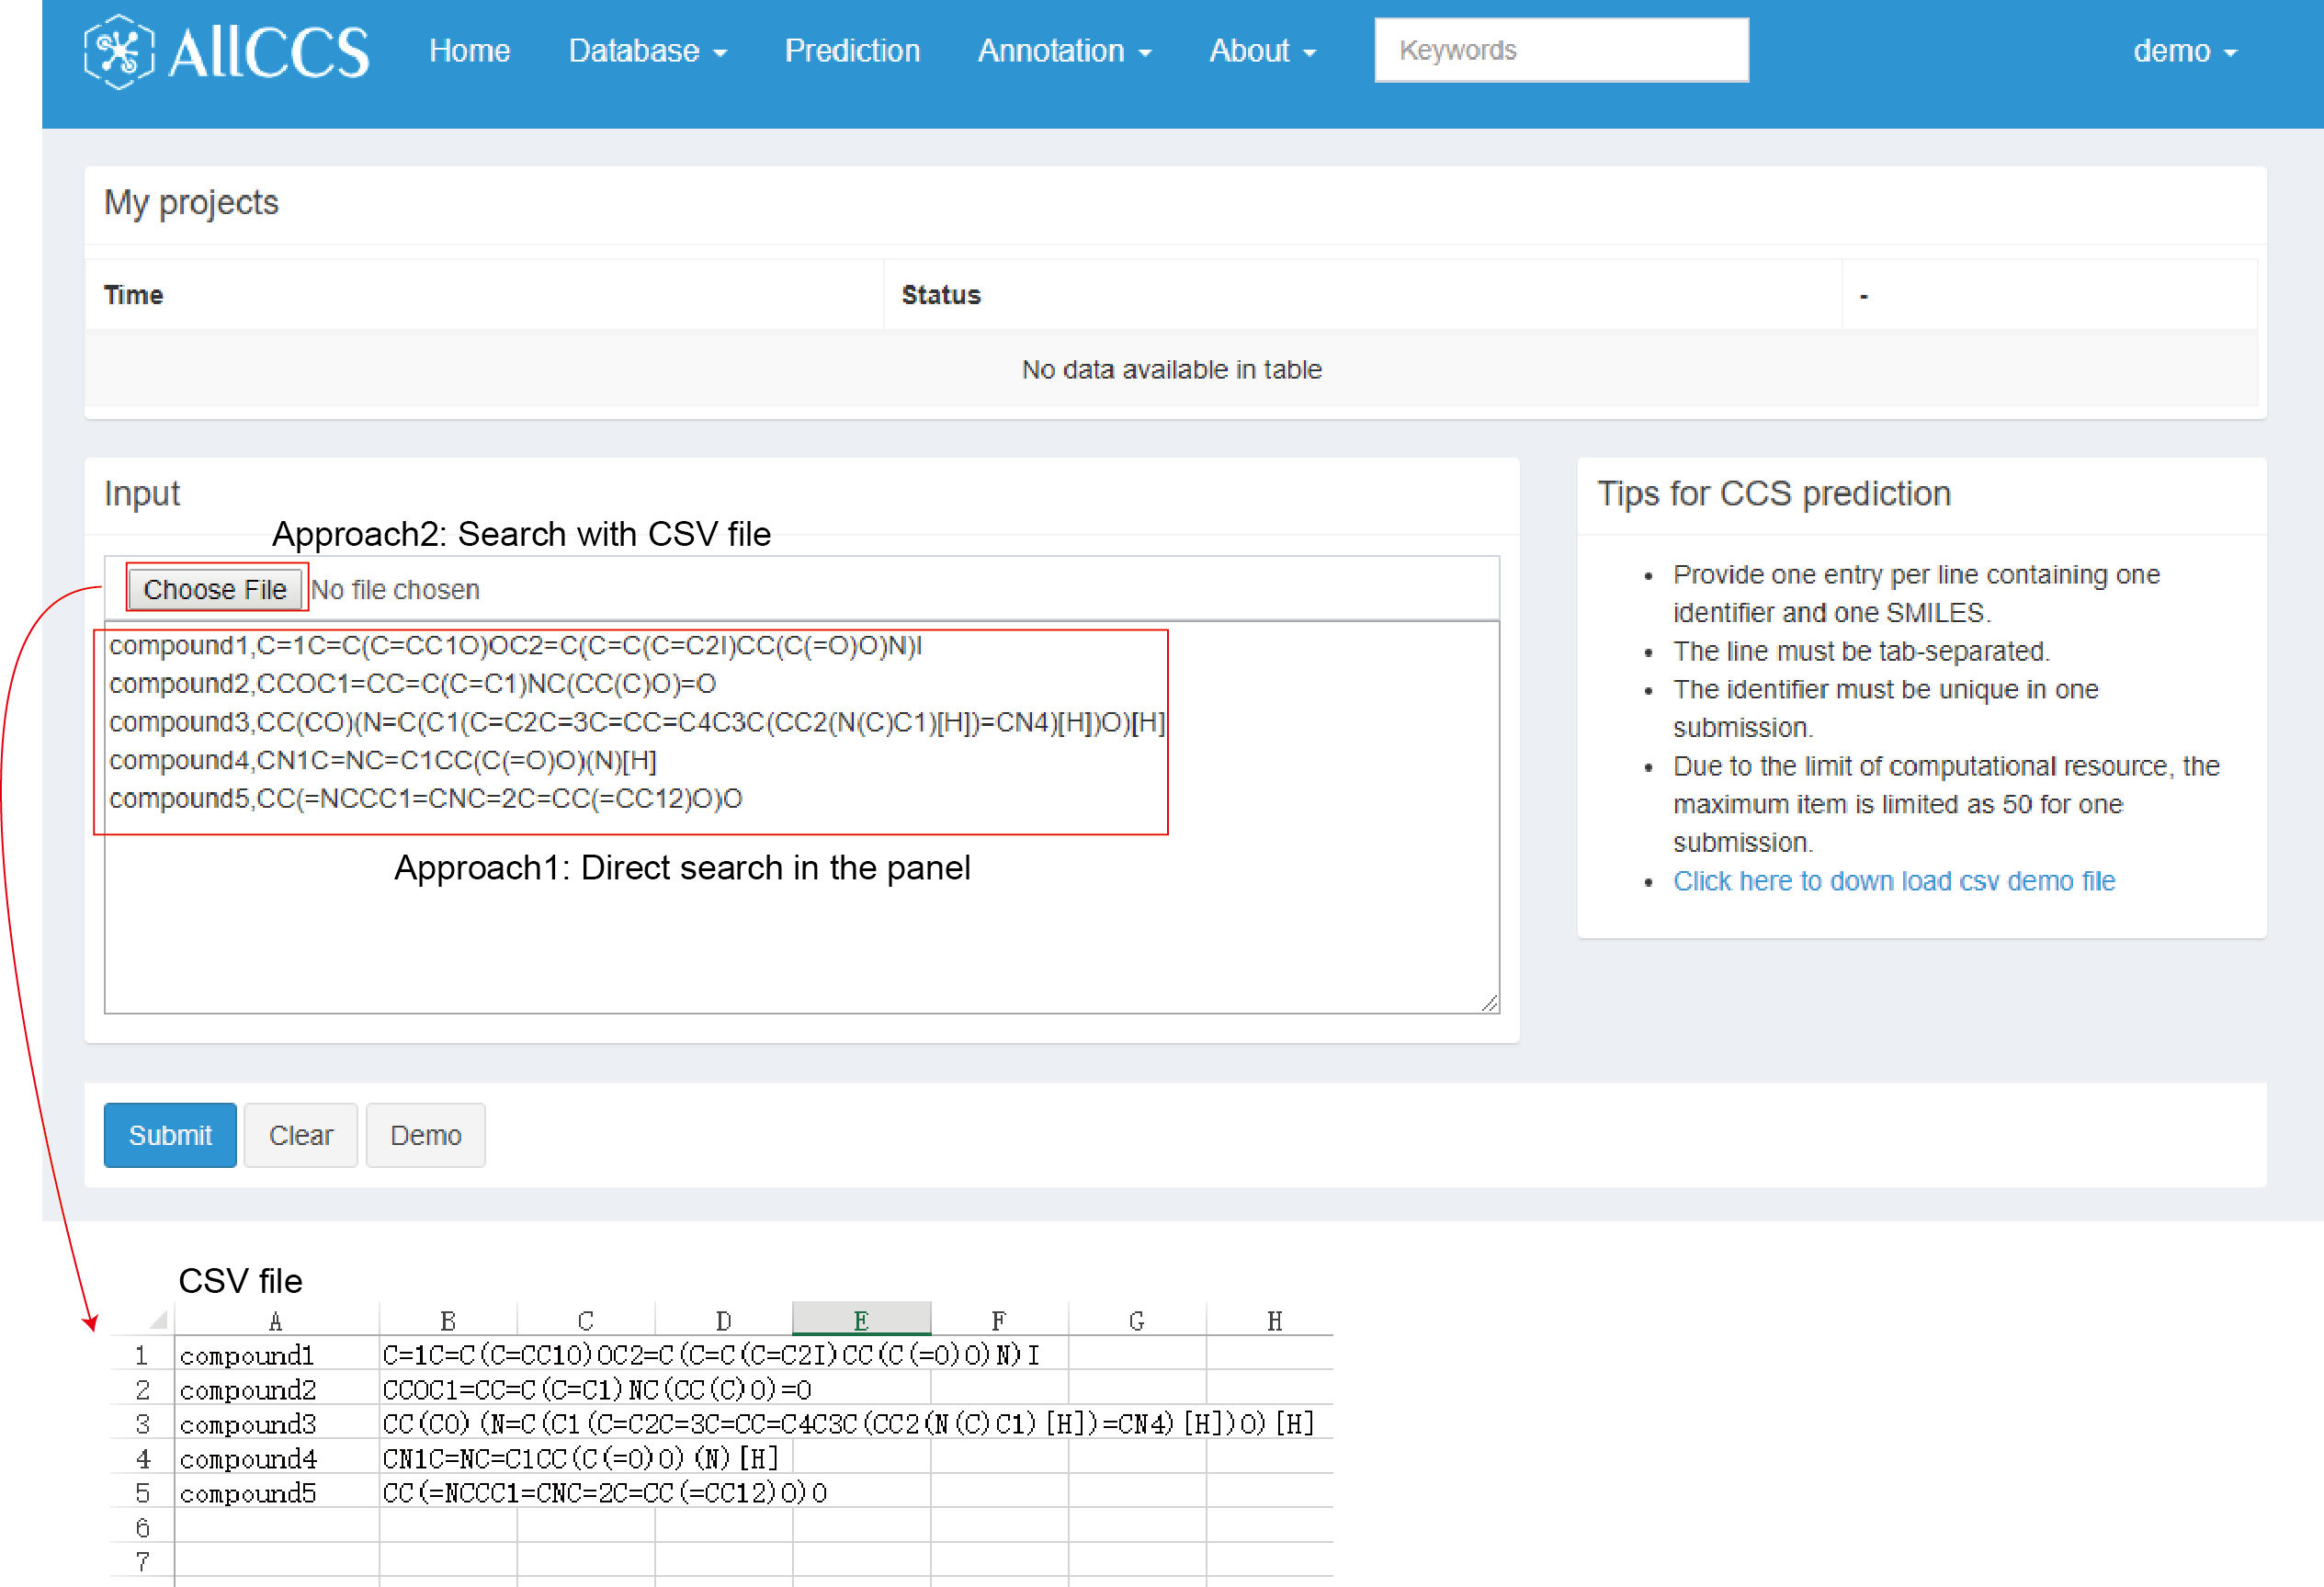
\includegraphics{images/chapter3/figure3.1prediction} 

}

\caption{CCS prediction}\label{fig:figure3d1}
\end{figure}

\subsection{Direct input in the panel}\label{chapter3d1d1}

Users can directly search in the panel with one entry per line
containing one identifier and one SMILES. When the input is complete,
click submit to get the predicted results.

\textbf{Note}:

\begin{itemize}
\tightlist
\item
  The line must be tab-separated.
\item
  The identifiers must be unique in one submission.
\item
  Due to the limit of computational resource, the maximum item is
  limited as 50 for one submission.
\end{itemize}

\subsection{Prediction with uploading CSV file}\label{chapter3d1d2}

It is also available for prediction by uploading a CSV file. Users can
download the CSV demo file, and the data format of the CSV file is
showed in the Figure \ref{fig:figure3d1}. The first column contains the
identifier of each SMILES and the second column is the corresponding
SMILES. The format of CSV file is same as the inputting panel. Please
note that the identifiers must be unique in one file, and the maximum
item is limited as \textbf{50} for one file.

\section{Result}\label{chapter3d2}

Results of user submissions are showed in the ``My projects'' panel
(Figure \ref{fig:figure3d2}).

\begin{figure}

{\centering 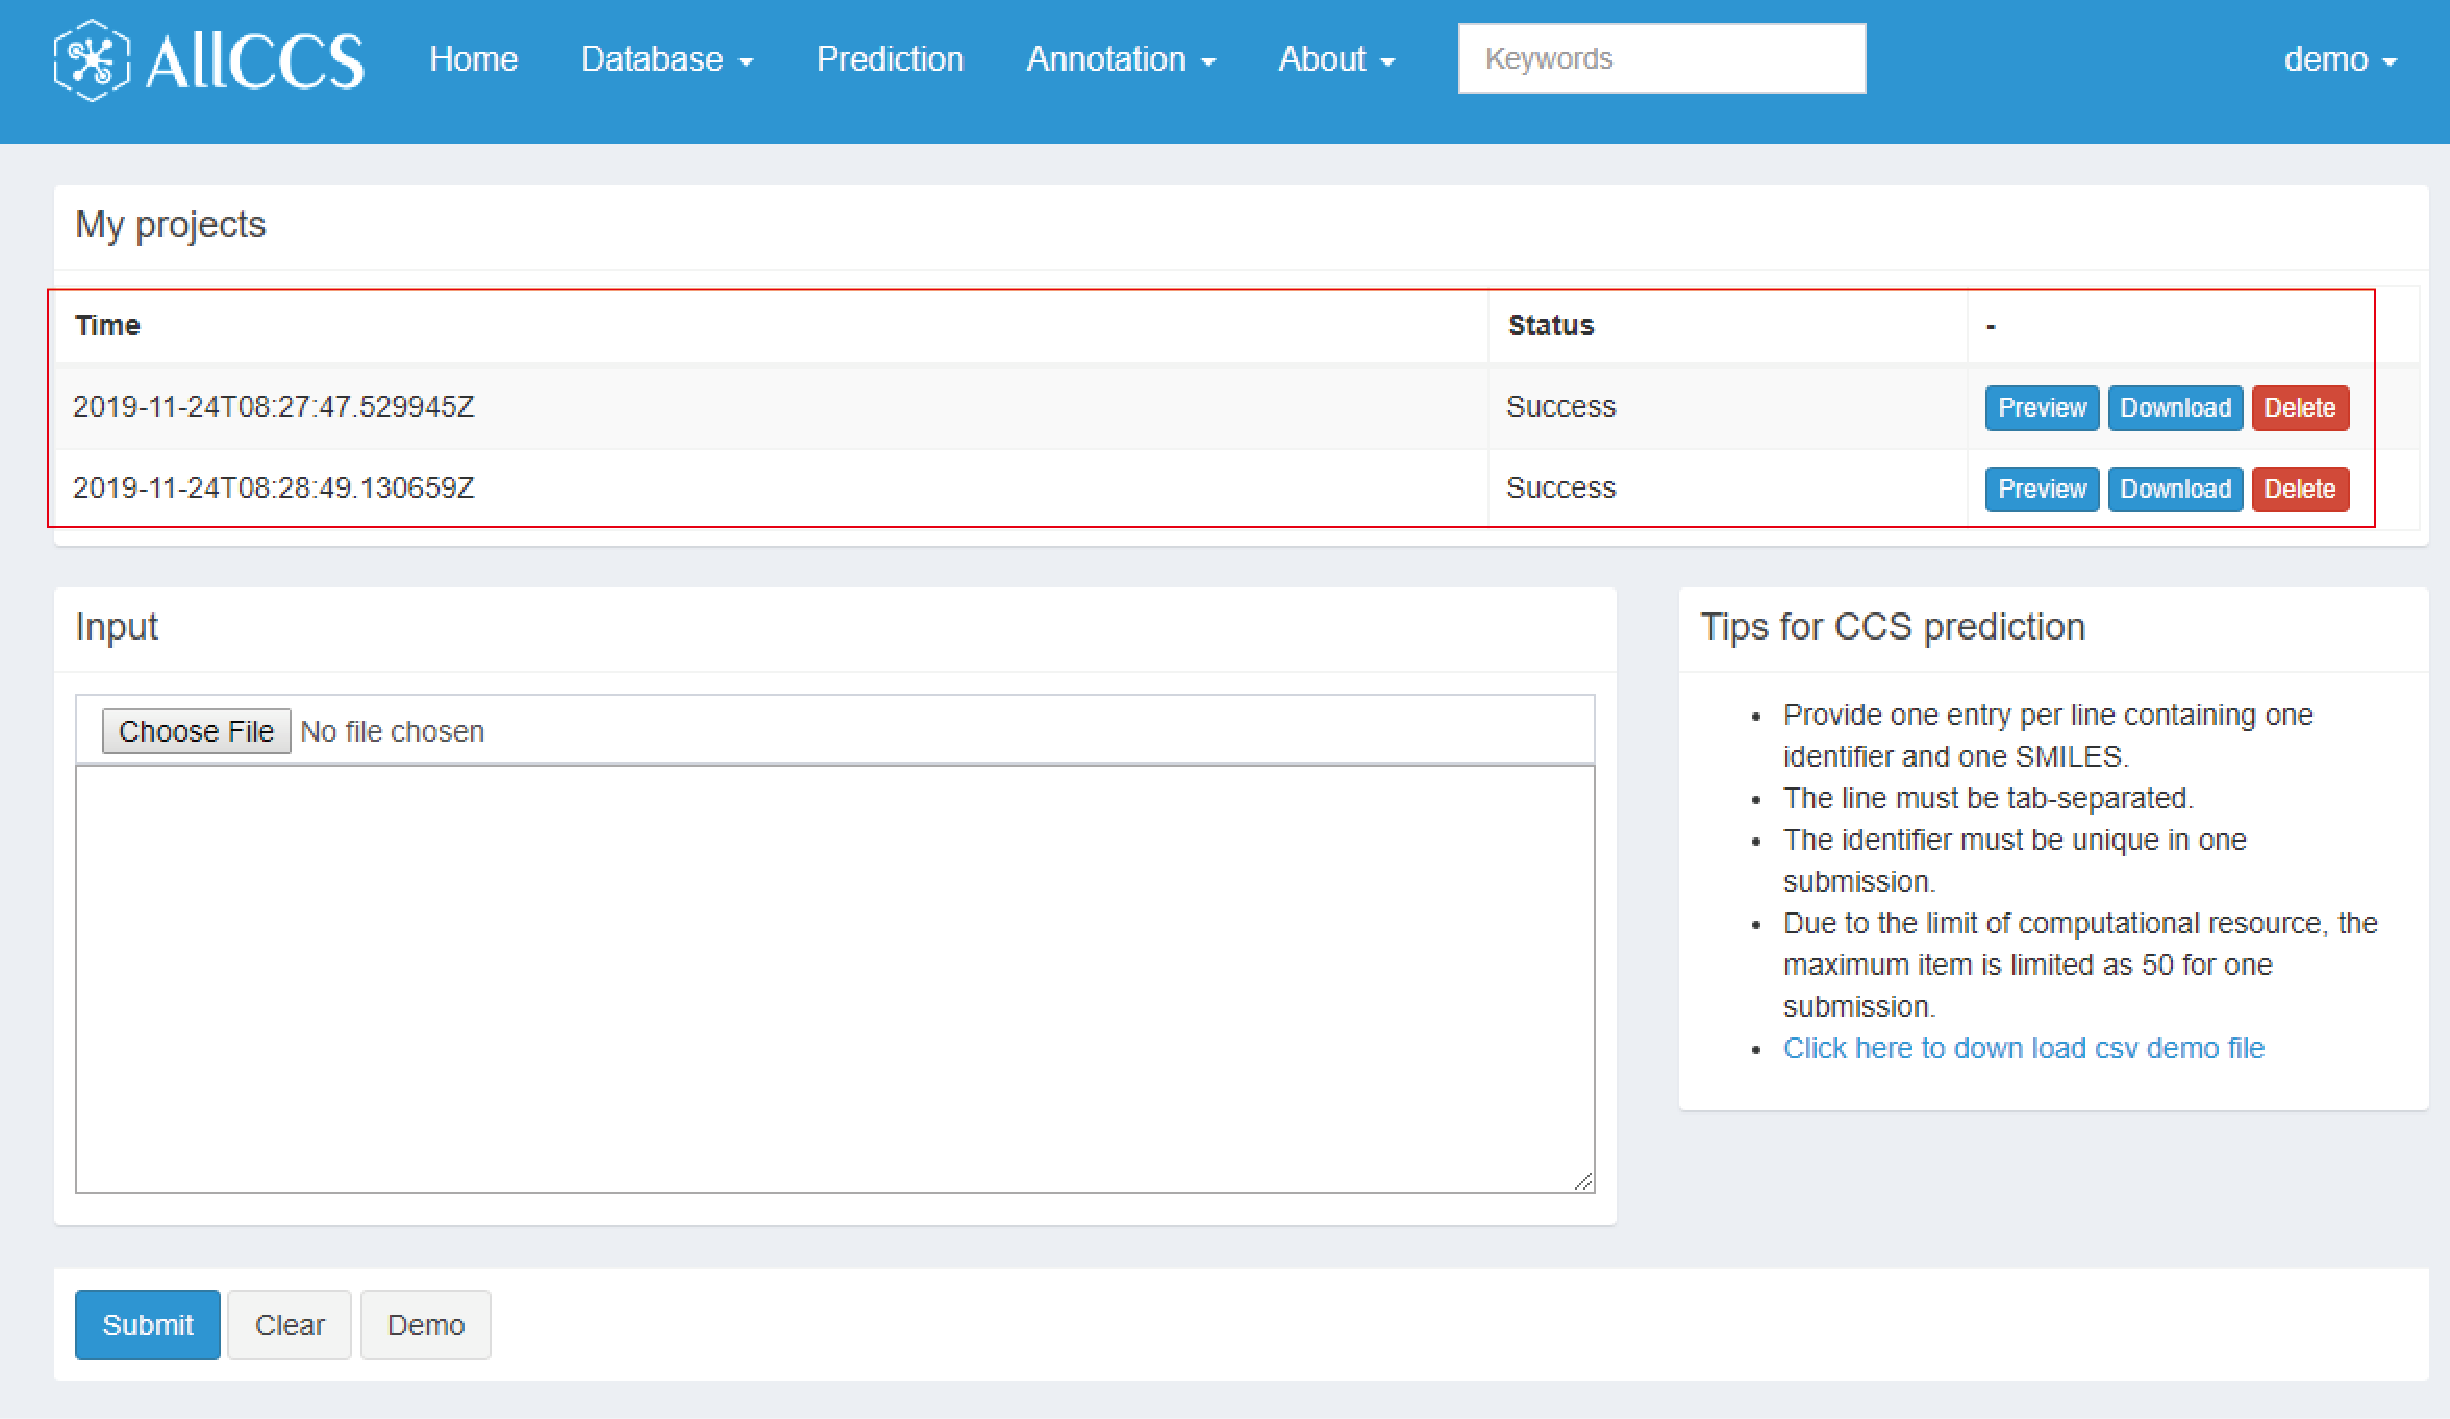
\includegraphics{images/chapter3/figure3.2prediction_result} 

}

\caption{CCS prediction results}\label{fig:figure3d2}
\end{figure}

With preview conditions, users can get the detailed result of inputted
SMILES (Figure \ref{fig:figure3d3}). Compounds entries would be sorted
by different adduct information. In below texts, it contains brief
information for each compound.

\begin{itemize}
\tightlist
\item
  \textbf{Name}: Consistent with the identifiers you input.
\item
  \textbf{SMILES}: SMILES structures.
\item
  \textbf{Monoisotopic mass}: Monoisotopic mass of structure
\item
  \textbf{Adduct}: The adduct form. AllCCS provides 7 adducts forms
  (Positive mode: {[}M+H{]}+, {[}M+Na{]}+, {[}M-H2O+H{]}+, {[}M+NH4{]}+;
  Negative mode: {[}M-H{]}-, {[}M+Na-2H{]}-, {[}M+HCOO{]}-).
\item
  \textbf{m/z}: The ratio of mass and charge
\item
  \textbf{Predicted CCS}: CCS value for the specific structure and
  adduct.
\item
  \textbf{RSS}: Representative structure similarity. See Section
  \ref{chapter2d2d4} for more information.
\item
  \textbf{Status}:

  \begin{itemize}
  \tightlist
  \item
    \textbf{Valid}: Successful prediction
  \item
    \textbf{Error1}: Invalid SMILES structure
  \item
    \textbf{Error2}: The mass range is out of the limitation (AllCCS
    only supports small compound CCS prediction with mass between
    60-1200).
  \end{itemize}
\end{itemize}

\begin{figure}

{\centering 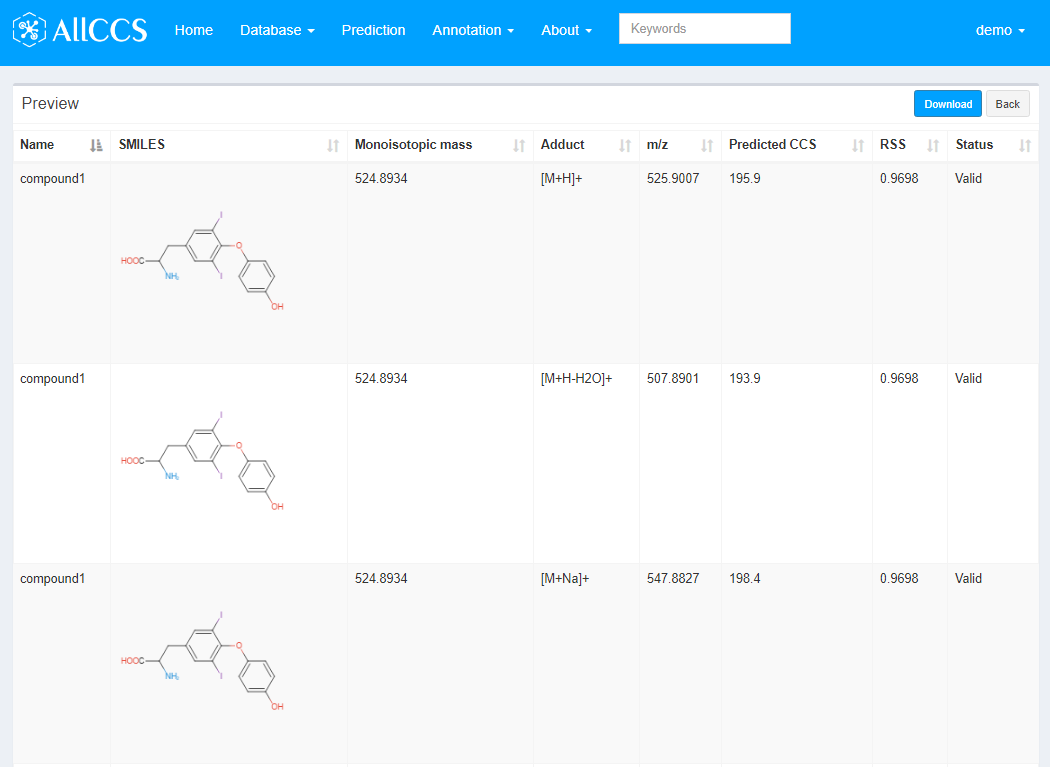
\includegraphics{images/chapter3/figure3.3preview_result} 

}

\caption{Preview results}\label{fig:figure3d3}
\end{figure}

Users can also click download to obtain CSV table which contains the
same information as preview results (Figure \ref{fig:figure3d4}).

\begin{figure}

{\centering 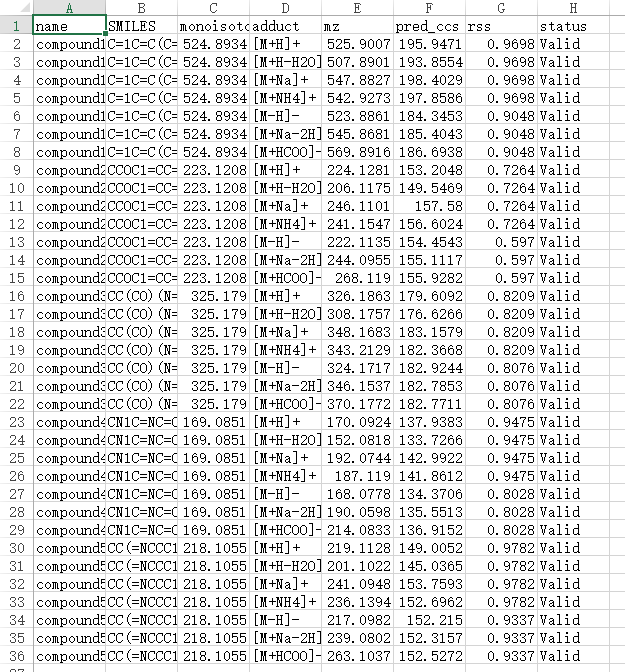
\includegraphics{images/chapter3/figure3.4download_result} 

}

\caption{Download results}\label{fig:figure3d4}
\end{figure}

\textbf{Note}:

\begin{itemize}
\tightlist
\item
  Due to the computation resource limitation, it allows up to 10
  projects one time in ``\emph{My projects panel}''. If users want to
  execute more projects, please delete previous projects.
\end{itemize}

\chapter{Metabolite Annotation}\label{chapter4}

The part provides an easy-to-use annotation function for unknown
features or compounds. It consists of two functions in this part. One is
feature match, which supports searching database with measured m/z and
CCS for annotation. The second function is candidate rank, which can be
in conjunct with any other annotation tools, such as MetFrag, CFM-ID,
MS-Finder, and SIRIUS etc. With the results from previously mentioned
tools, and inputting experimental m/z and experimental CCS, users can
filter/re-rank candidates for more accurate annotation.

\section{Feature to candidates (Feature match)}\label{chapter4d1}

Feature match function provides a simple and straightforward way to
annotate features with experimental m/z and CCS in the AllCCS database.
There are several annotation conditions set in this part (Figure
\ref{fig:figure4d1}).

\begin{figure}

{\centering 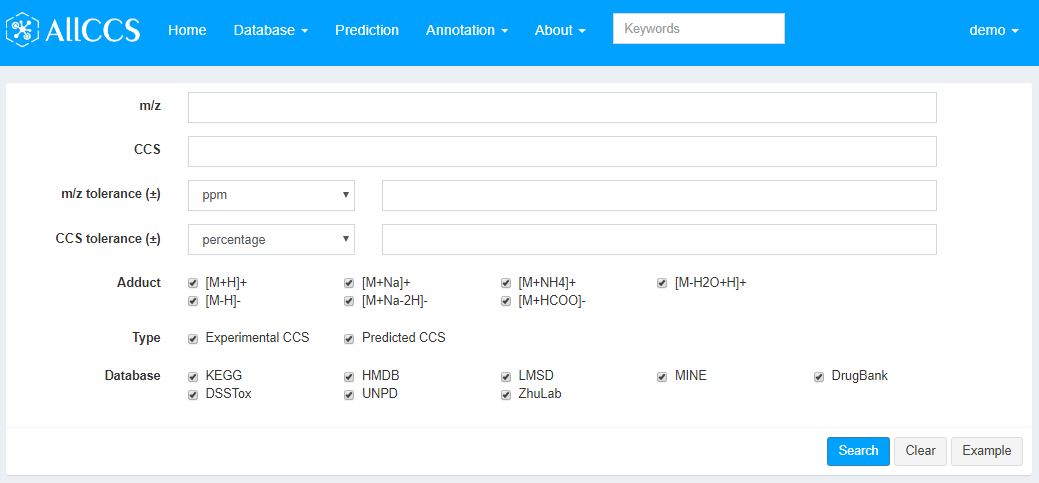
\includegraphics{images/chapter4/figure4.1} 

}

\caption{Feature annotation}\label{fig:figure4d1}
\end{figure}

\begin{itemize}
\tightlist
\item
  \textbf{m/z}: Experimental m/z of your interested peaks.
\item
  \textbf{CCS}: Experimental CCS of your interested peaks.
\item
  \textbf{m/z tolerance (±)}: The tolerance between experimental m/z and
  theoretical m/z in database. Users can choose ppm or Dalton as unit.
\item
  \textbf{CCS tolerance (±)}: The tolerance between experimental CCS and
  theoretical CCS in database. Users can choose percentage or Å2 as
  unit.
\item
  \textbf{Adduct}: Match with the checked adduct forms that exist in the
  database.
\item
  \textbf{Type}: Match with the checked CCS type in the database,
  including Experimental CCS, Predicted CCS (See Section
  \ref{chapter2d1}).
\item
  \textbf{Database}: Match with the checked database. It includes 8
  compound structure sources (See Section \ref{chapter2d1}).
\end{itemize}

The match results are as follows (Figure \ref{fig:figure4d2}). The
results contain brief information for each compound as section 2.1
Compound Browser mentioned.

Users can check the interested compounds in the last column. Click the
download option, you could download a CSV table containing the
information of you checked compounds (Figure \ref{fig:figure4d2}).

\textbf{Note}:

\begin{itemize}
\tightlist
\item
  Download function supports up to 100 items for one time.
\end{itemize}

\begin{figure}

{\centering 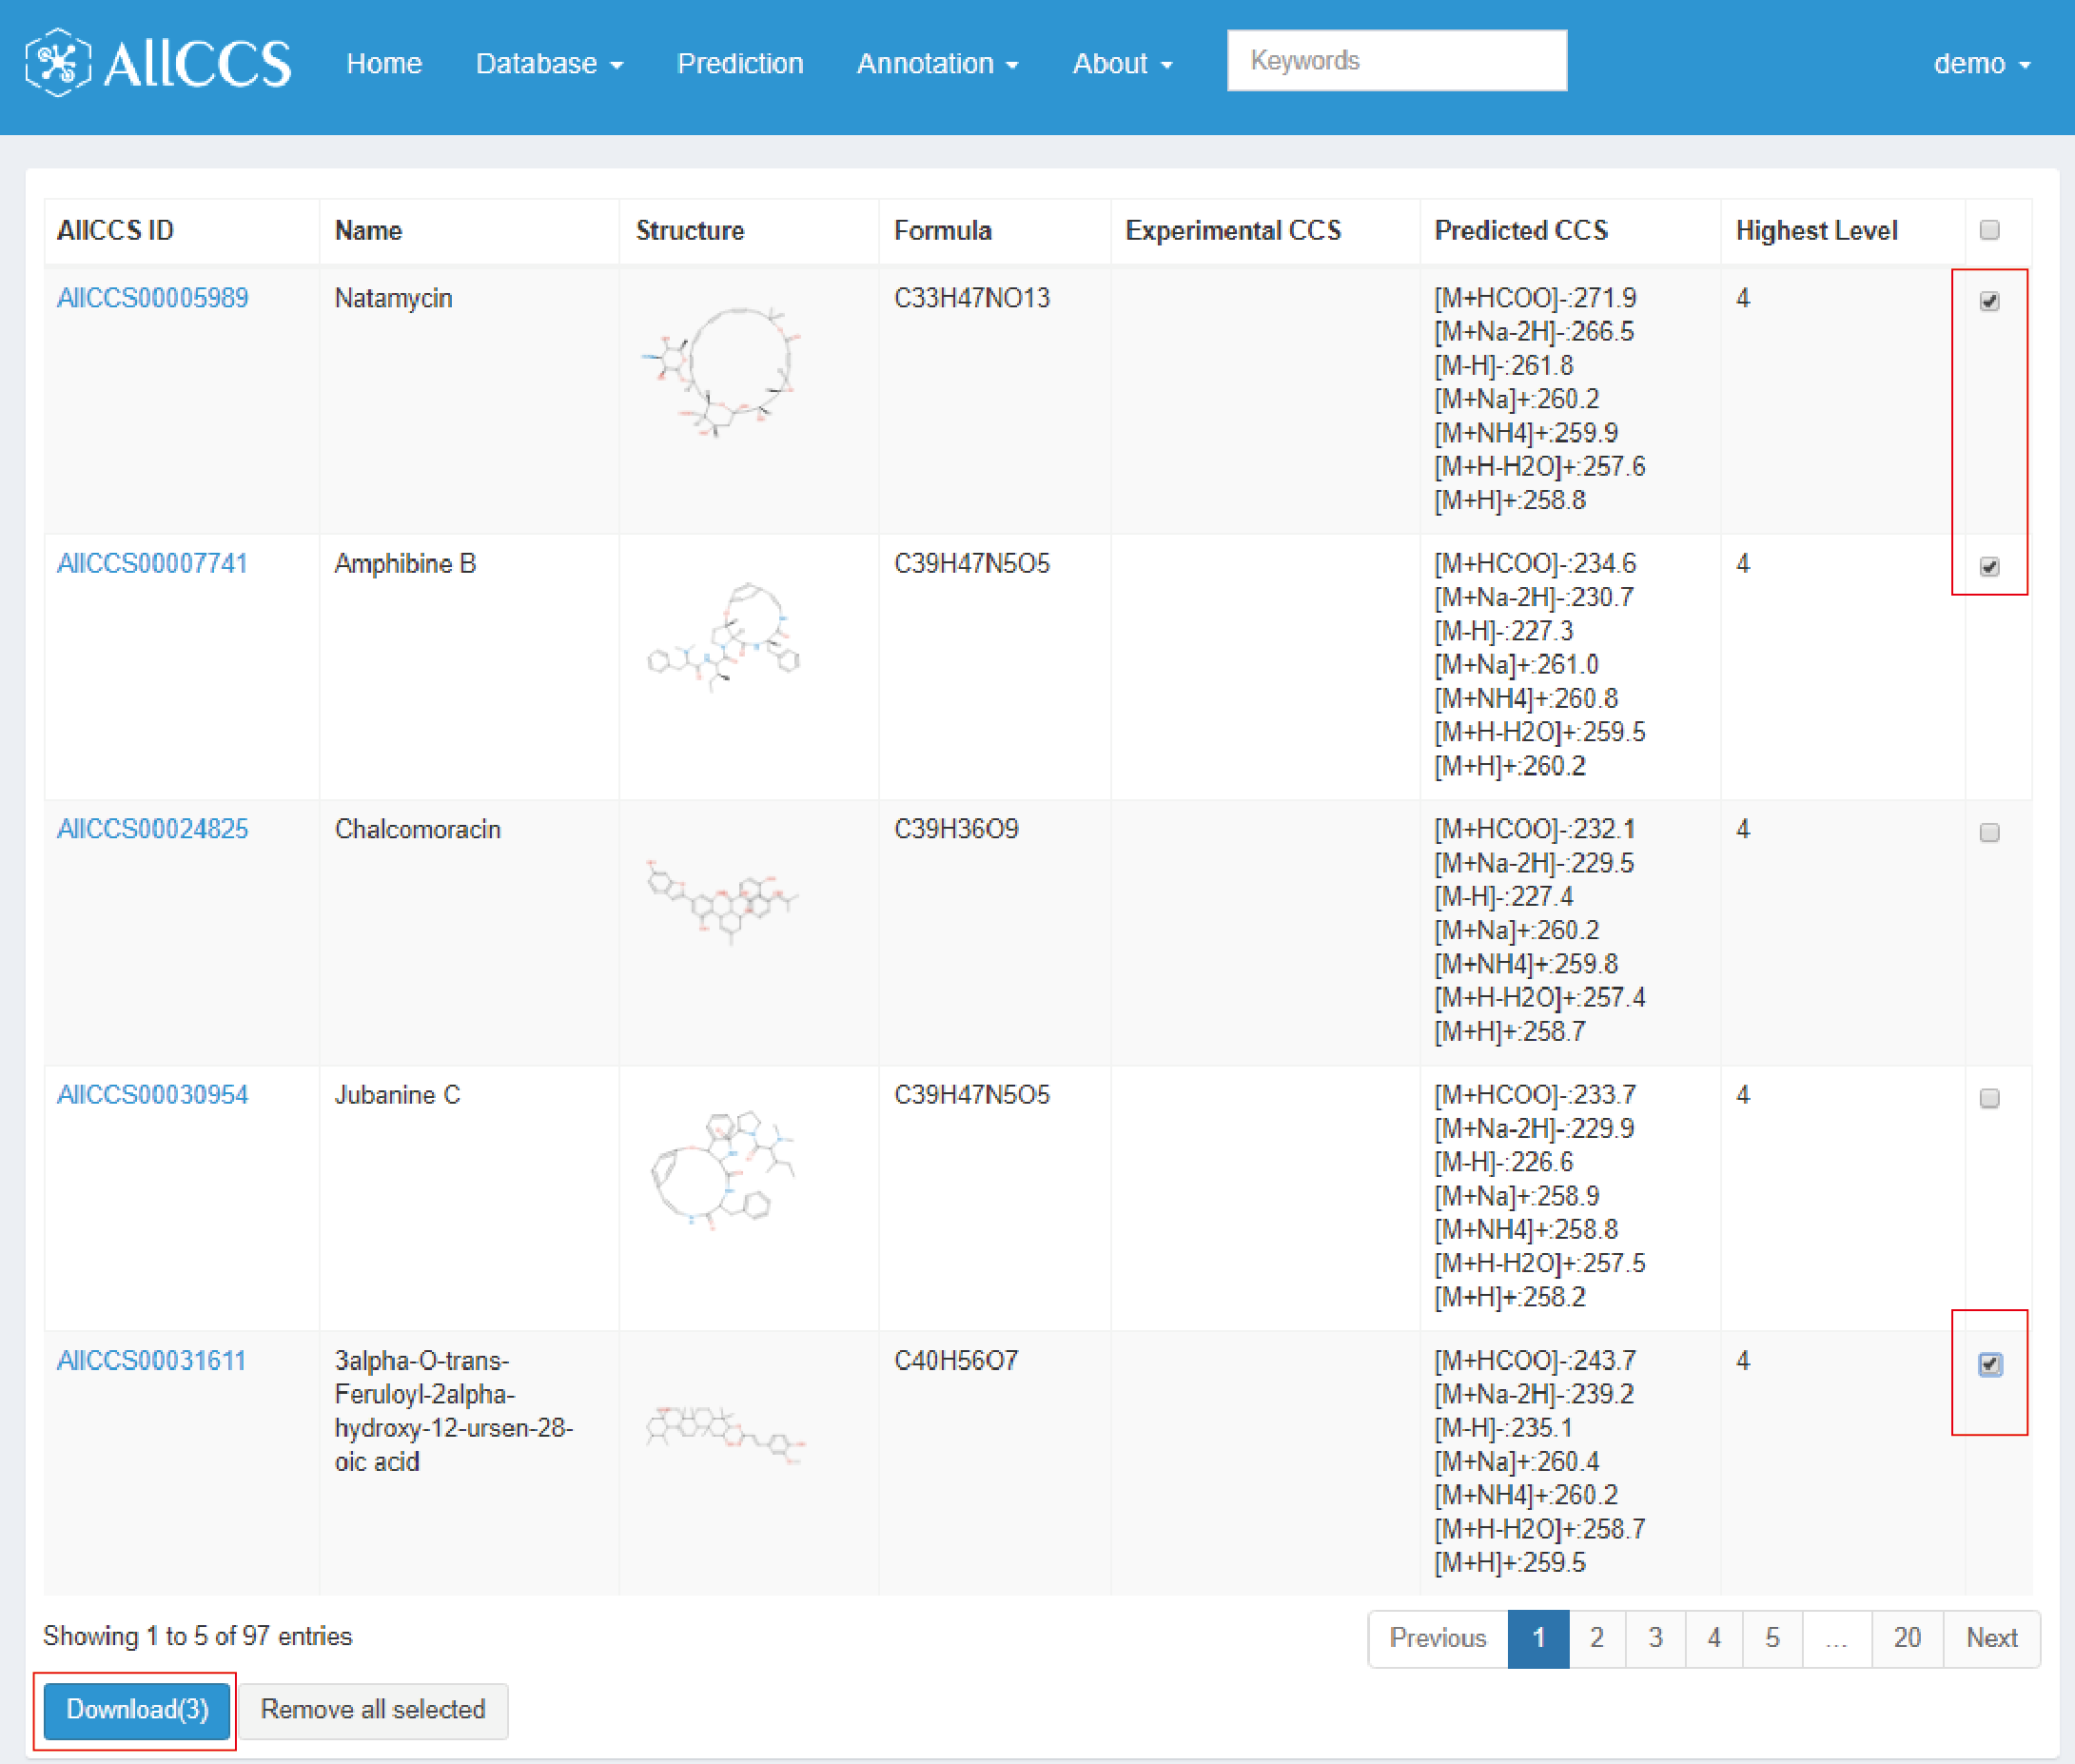
\includegraphics{images/chapter4/figure4.2feature_match} 

}

\caption{Feature match results}\label{fig:figure4d2}
\end{figure}

\section{Complement to MS/MS result (Candidate rank)}\label{chapter4d2}

The candidate rank function supports filtering/re-rank candidates with
inputted candidate list. This function could be in conjunct with any
other in-silico MS/MS tools like MetFrag, CFM-ID, MS-Finder, and SIRIUS
etc. Specifically, it has two rank types: \textbf{CCS filtering} and
\textbf{CCS scoring}. CCS filtering excludes candidates which CCS errors
(comparing with predicted CCS values) beyond the pre-defined cutoff
value. CCS scoring generates an integrated score for each candidate with
custom weights of CCS score (The detail is some with our previous
publication - LipidIMMS Analyzer \citep{reference9}) and MS/MS score.
With CCS filtering or scoring, it can provide more credible results.

\subsection{Data preparation}\label{chapter4d2d1}

The MS/MS results (CSV file) generated from other tools should be
modified as specific format. A demo data is showed in Figure
\ref{fig:figure4d3}. It should include 7 columns with specific names
(``rank'', ``name'', ``smiles'', ``inchikey'', ``adduct'', ``score'').
The definitions of each column are given as follows:

\begin{figure}

{\centering 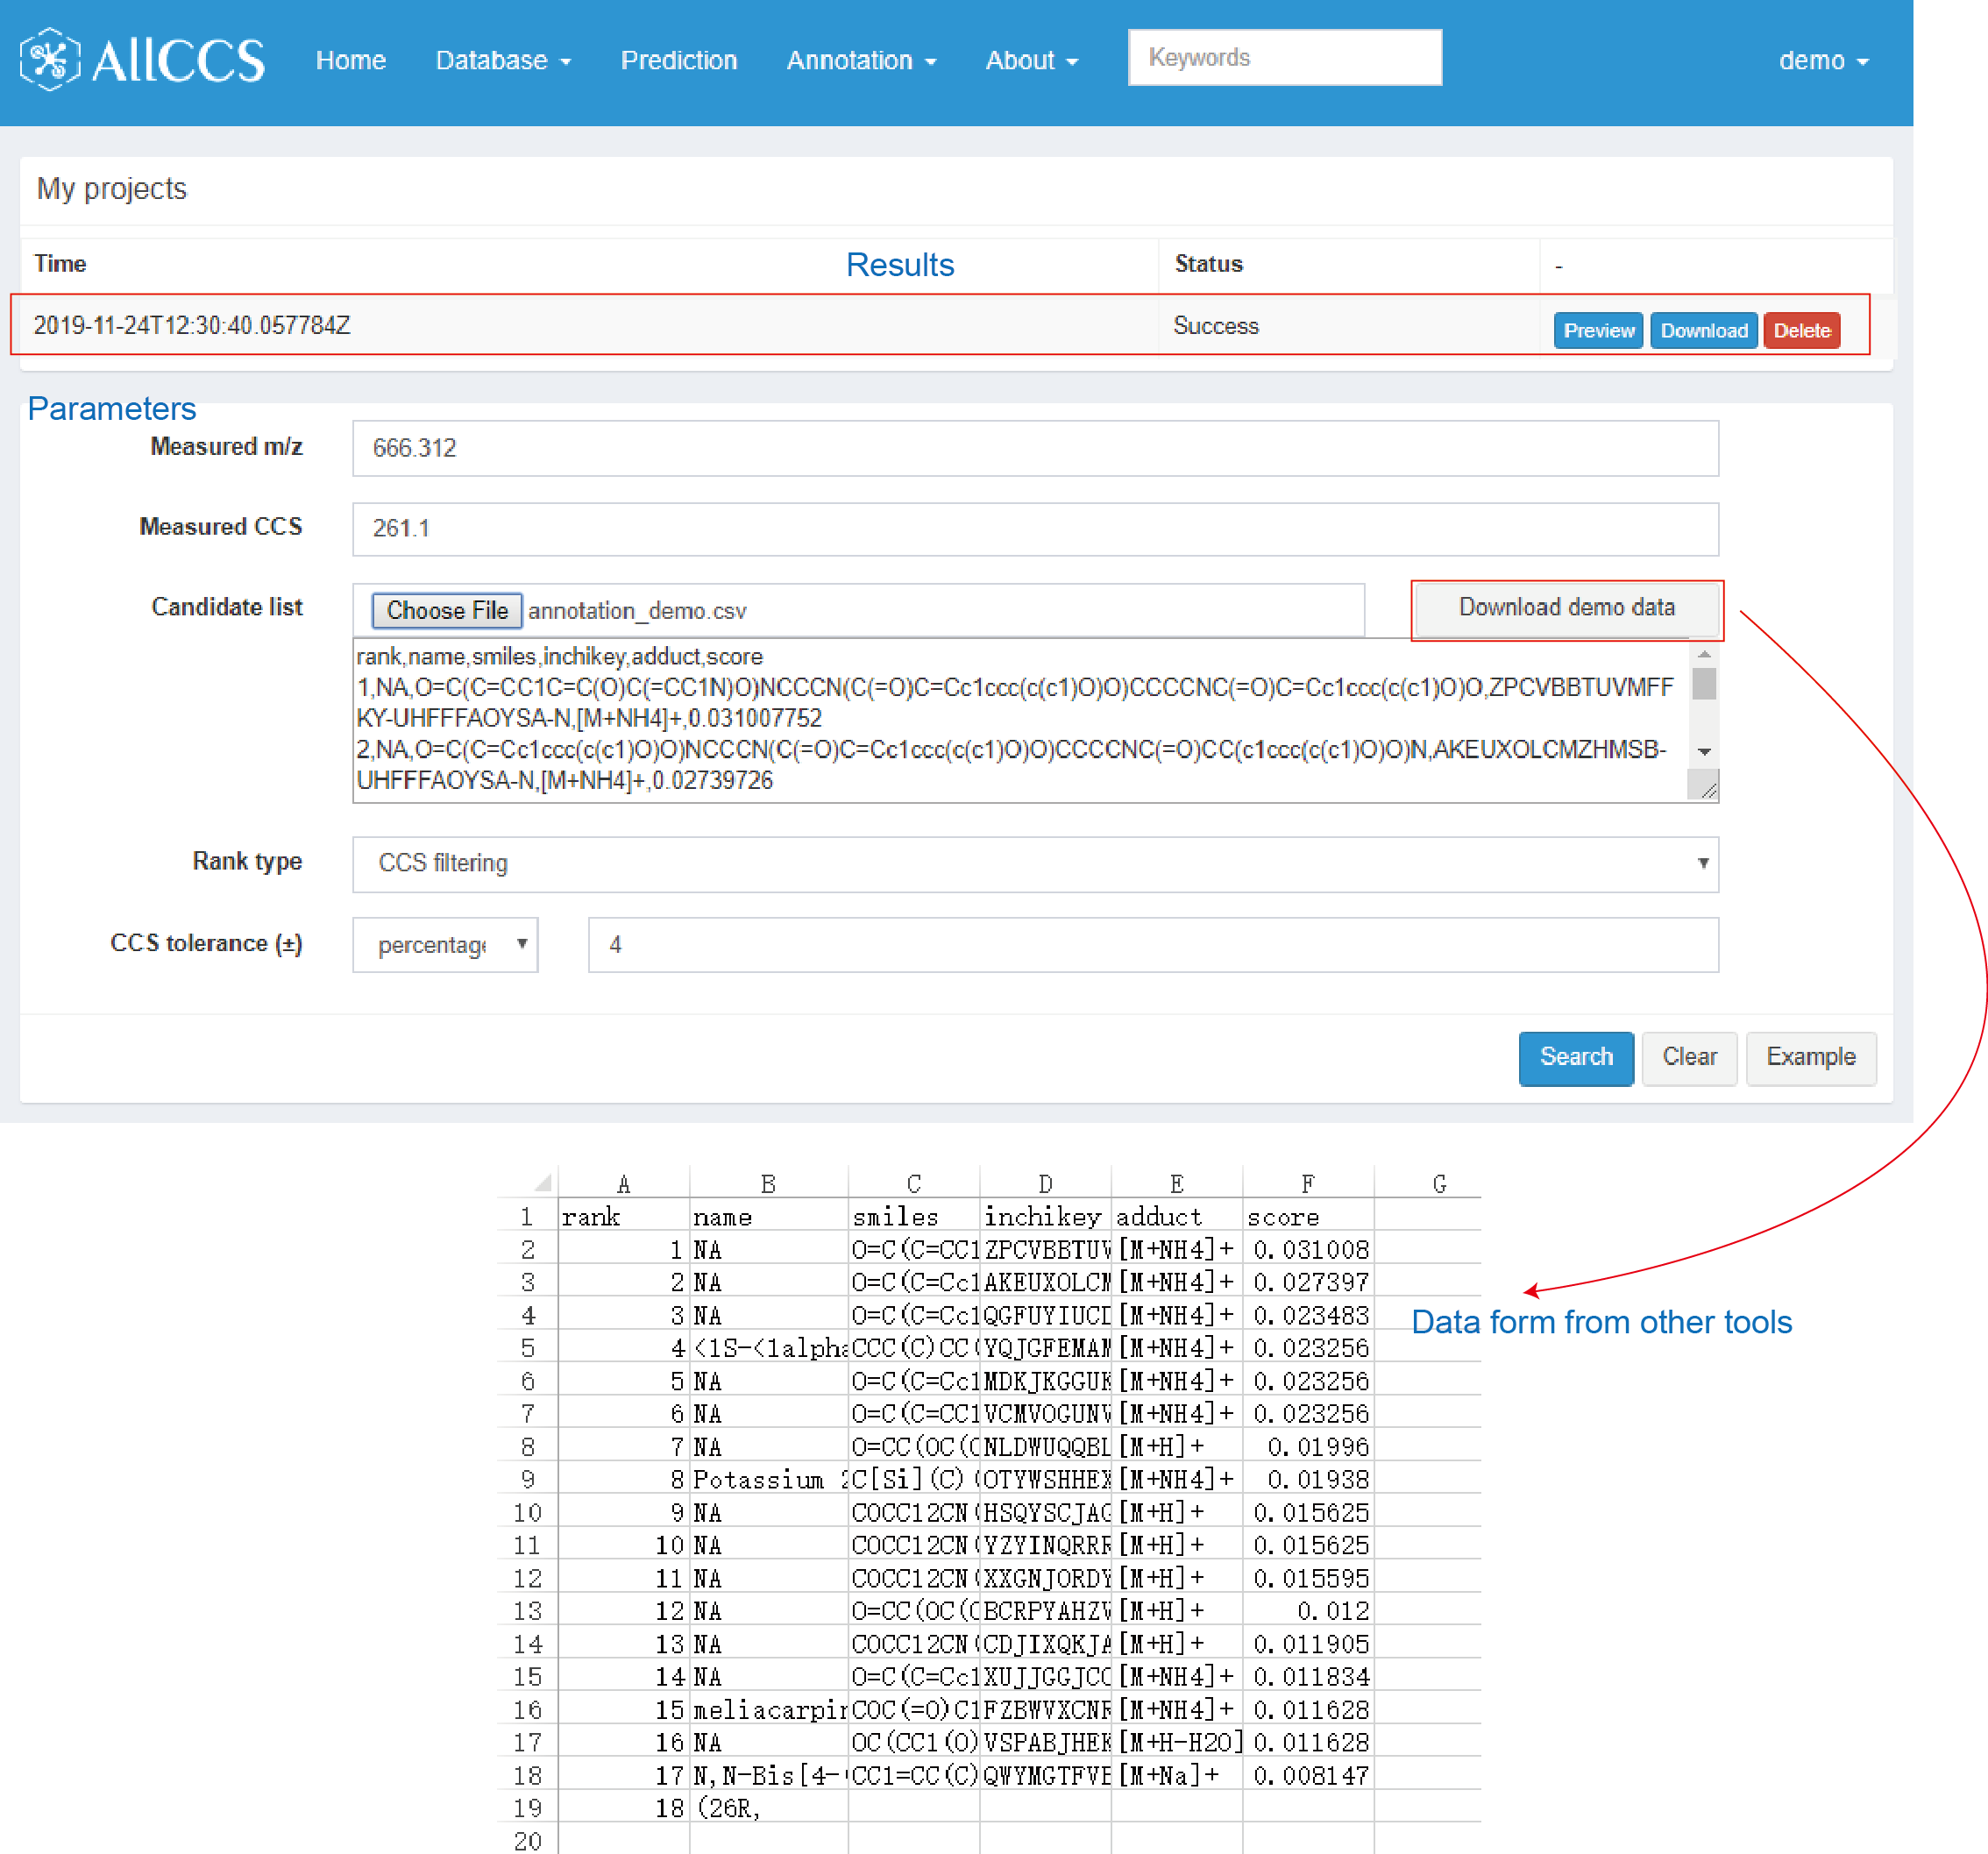
\includegraphics{images/chapter4/figure4.3candidate_rank} 

}

\caption{Candidate rank function}\label{fig:figure4d3}
\end{figure}

\begin{itemize}
\tightlist
\item
  \textbf{rank}: The first column in the CSV table. It is the score rank
  from other tools (e.g.~MetFrag, CFM-ID, MS-FINDER, SIRIUS etc).
\item
  \textbf{name}: The second column in the CSV table. Compound names of
  candidates.
\item
  \textbf{smiles}: The third column in the CSV table. SMILES structures
  of candidates.
\item
  \textbf{inchikey}: The fourth column in the CSV table. InChIKey
  identifier of candidates.
\item
  \textbf{adduct}: The fifth column in the CSV table. Adduct form of
  candidates. Please note that it only supports 7 common adducts
  (Positive mode, {[}M+H{]}+, {[}M+Na{]}+, {[}M+NH4{]}+, {[}M-H2O+H{]}+;
  Negative mode, {[}M-H{]}-, {[}M+Na-2H{]}-, {[}M+HCOO{]}-).
\item
  \textbf{score}: The sixth column in the CSV table. The MS/MS match
  score generated in in-silico MS/MS tools.
\end{itemize}

\textbf{Note}:

\begin{itemize}
\tightlist
\item
  The inputted CSV file should have the same column name with demo data.
\item
  The column order should be keep same with demo data.
\end{itemize}

\subsection{Parameter setting}\label{chapter4d2d2}

In the candidates rank function, users can get more reliable results by
adjusting parameters according to their experiments. The candidate rank
function contains parameters as follows:

\begin{itemize}
\tightlist
\item
  \textbf{Measured m/z}: Experimental m/z of corresponding feature.
\item
  \textbf{Measured CCS}: Experimental CCS of corresponding feature.
\item
  \textbf{Candidate list}: A CSV file of candidate (See Section
  \ref{chapter4d2d1}).
\item
  \textbf{Rank type}: It consists of CCS filtering and CCS scoring. When
  choosing CCS filtering, the next option is CCS tolerance (Figure
  \ref{fig:figure4d3}). It will filter the results that out of the
  pre-defined CCS tolerance. If you choose CCS scoring, the follow
  options are showed as Figure Figure \ref{fig:figure4d4}. It consists
  of Minimum tolerance, Maximum tolerance, CCS weight, and MS/MS weight.
\item
  \textbf{CCS tolerance (±)}: This parameter is available in CCS
  filtering. The tolerance between experimental CCS and theoretical CCS
  in database. Users can choose percentage or Å2 as unit.
\item
  \textbf{Minimum tolerance (\%)}: This parameter is available in CCS
  scoring. If error is within the tolerance, CCS match score equals to
  1. Range: 0-10.
\item
  \textbf{Maximum tolerance (\%)}: This parameter is available in CCS
  scoring. If error is larger than the tolerance, CCS match score equals
  to 0, and lipid candidates will be removed. Range: 0-20.
\item
  \textbf{CCS weight}: This parameter is available in CCS scoring. The
  CCS match score weight to calculate integrated score.
\item
  \textbf{MS/MS weight}: This parameter is available in CCS scoring. The
  MS/MS match score weight to calculate integrated score.
\end{itemize}

\begin{figure}

{\centering 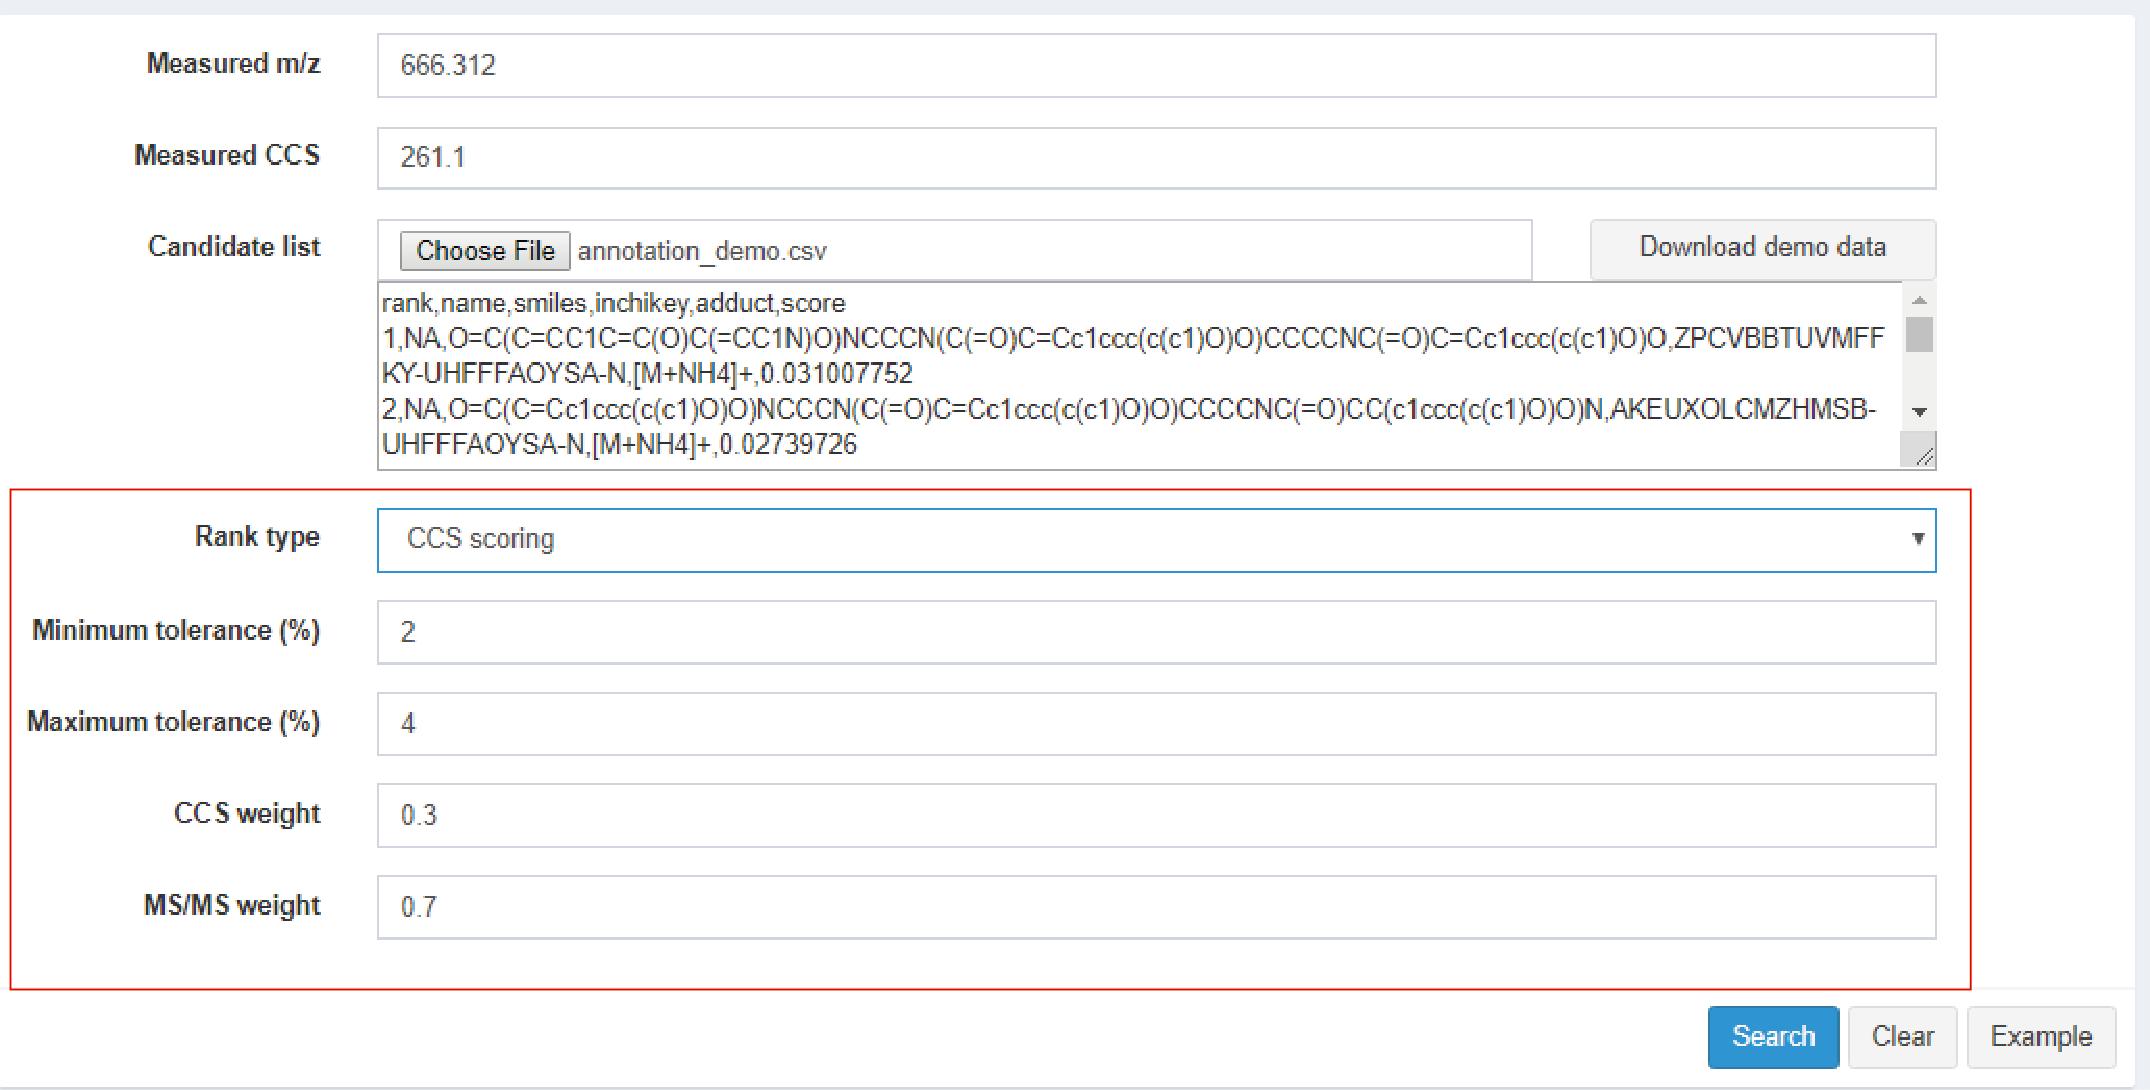
\includegraphics{images/chapter4/figure4.4CCS_scoring} 

}

\caption{CCS scoring}\label{fig:figure4d4}
\end{figure}

\subsection{Results}\label{chapter4d2d3}

Results of user submission are showed in the ``My projects'' panel
(Figure \ref{fig:figure4d2}).

\subsubsection{CCS filtering}\label{chapter4d2d3d1}

Users can get the detailed information of candidates by clicking the
browser button (Figure \ref{fig:figure4d5}). In below text, it contains
brief information for each candidate.

\begin{itemize}
\tightlist
\item
  \textbf{Rank}: The new rank after filtering with CCS.
\item
  \textbf{Name}: Consistent with the name in candidate list (see Section
  \ref{chapter4d2d1}).
\item
  \textbf{SMILES}: Consistent with the smiles in candidate list (see
  Section \ref{chapter4d2d1}).
\item
  \textbf{InChIKey}: Consistent with the inchikey in candidate list (see
  Section \ref{chapter4d2d1}).
\item
  \textbf{Adduct}: Consistent with the adduct in candidate list (see
  Section \ref{chapter4d2d1}).
\item
  \textbf{MS/MS score}: Consistent with the score in candidate list (see
  Section \ref{chapter4d2d1}).
\item
  \textbf{MS/MS rank}: Consistent with the rank in candidate list (see
  Section \ref{chapter4d2d1}).
\item
  \textbf{Predicted CCS (Å2)}: The predicted CCS with SMILES and
  InChIKey.
\end{itemize}

Users can also click download to obtain CSV table which contains the
same information as preview results (Figure \ref{fig:figure4d5}).

\begin{figure}

{\centering 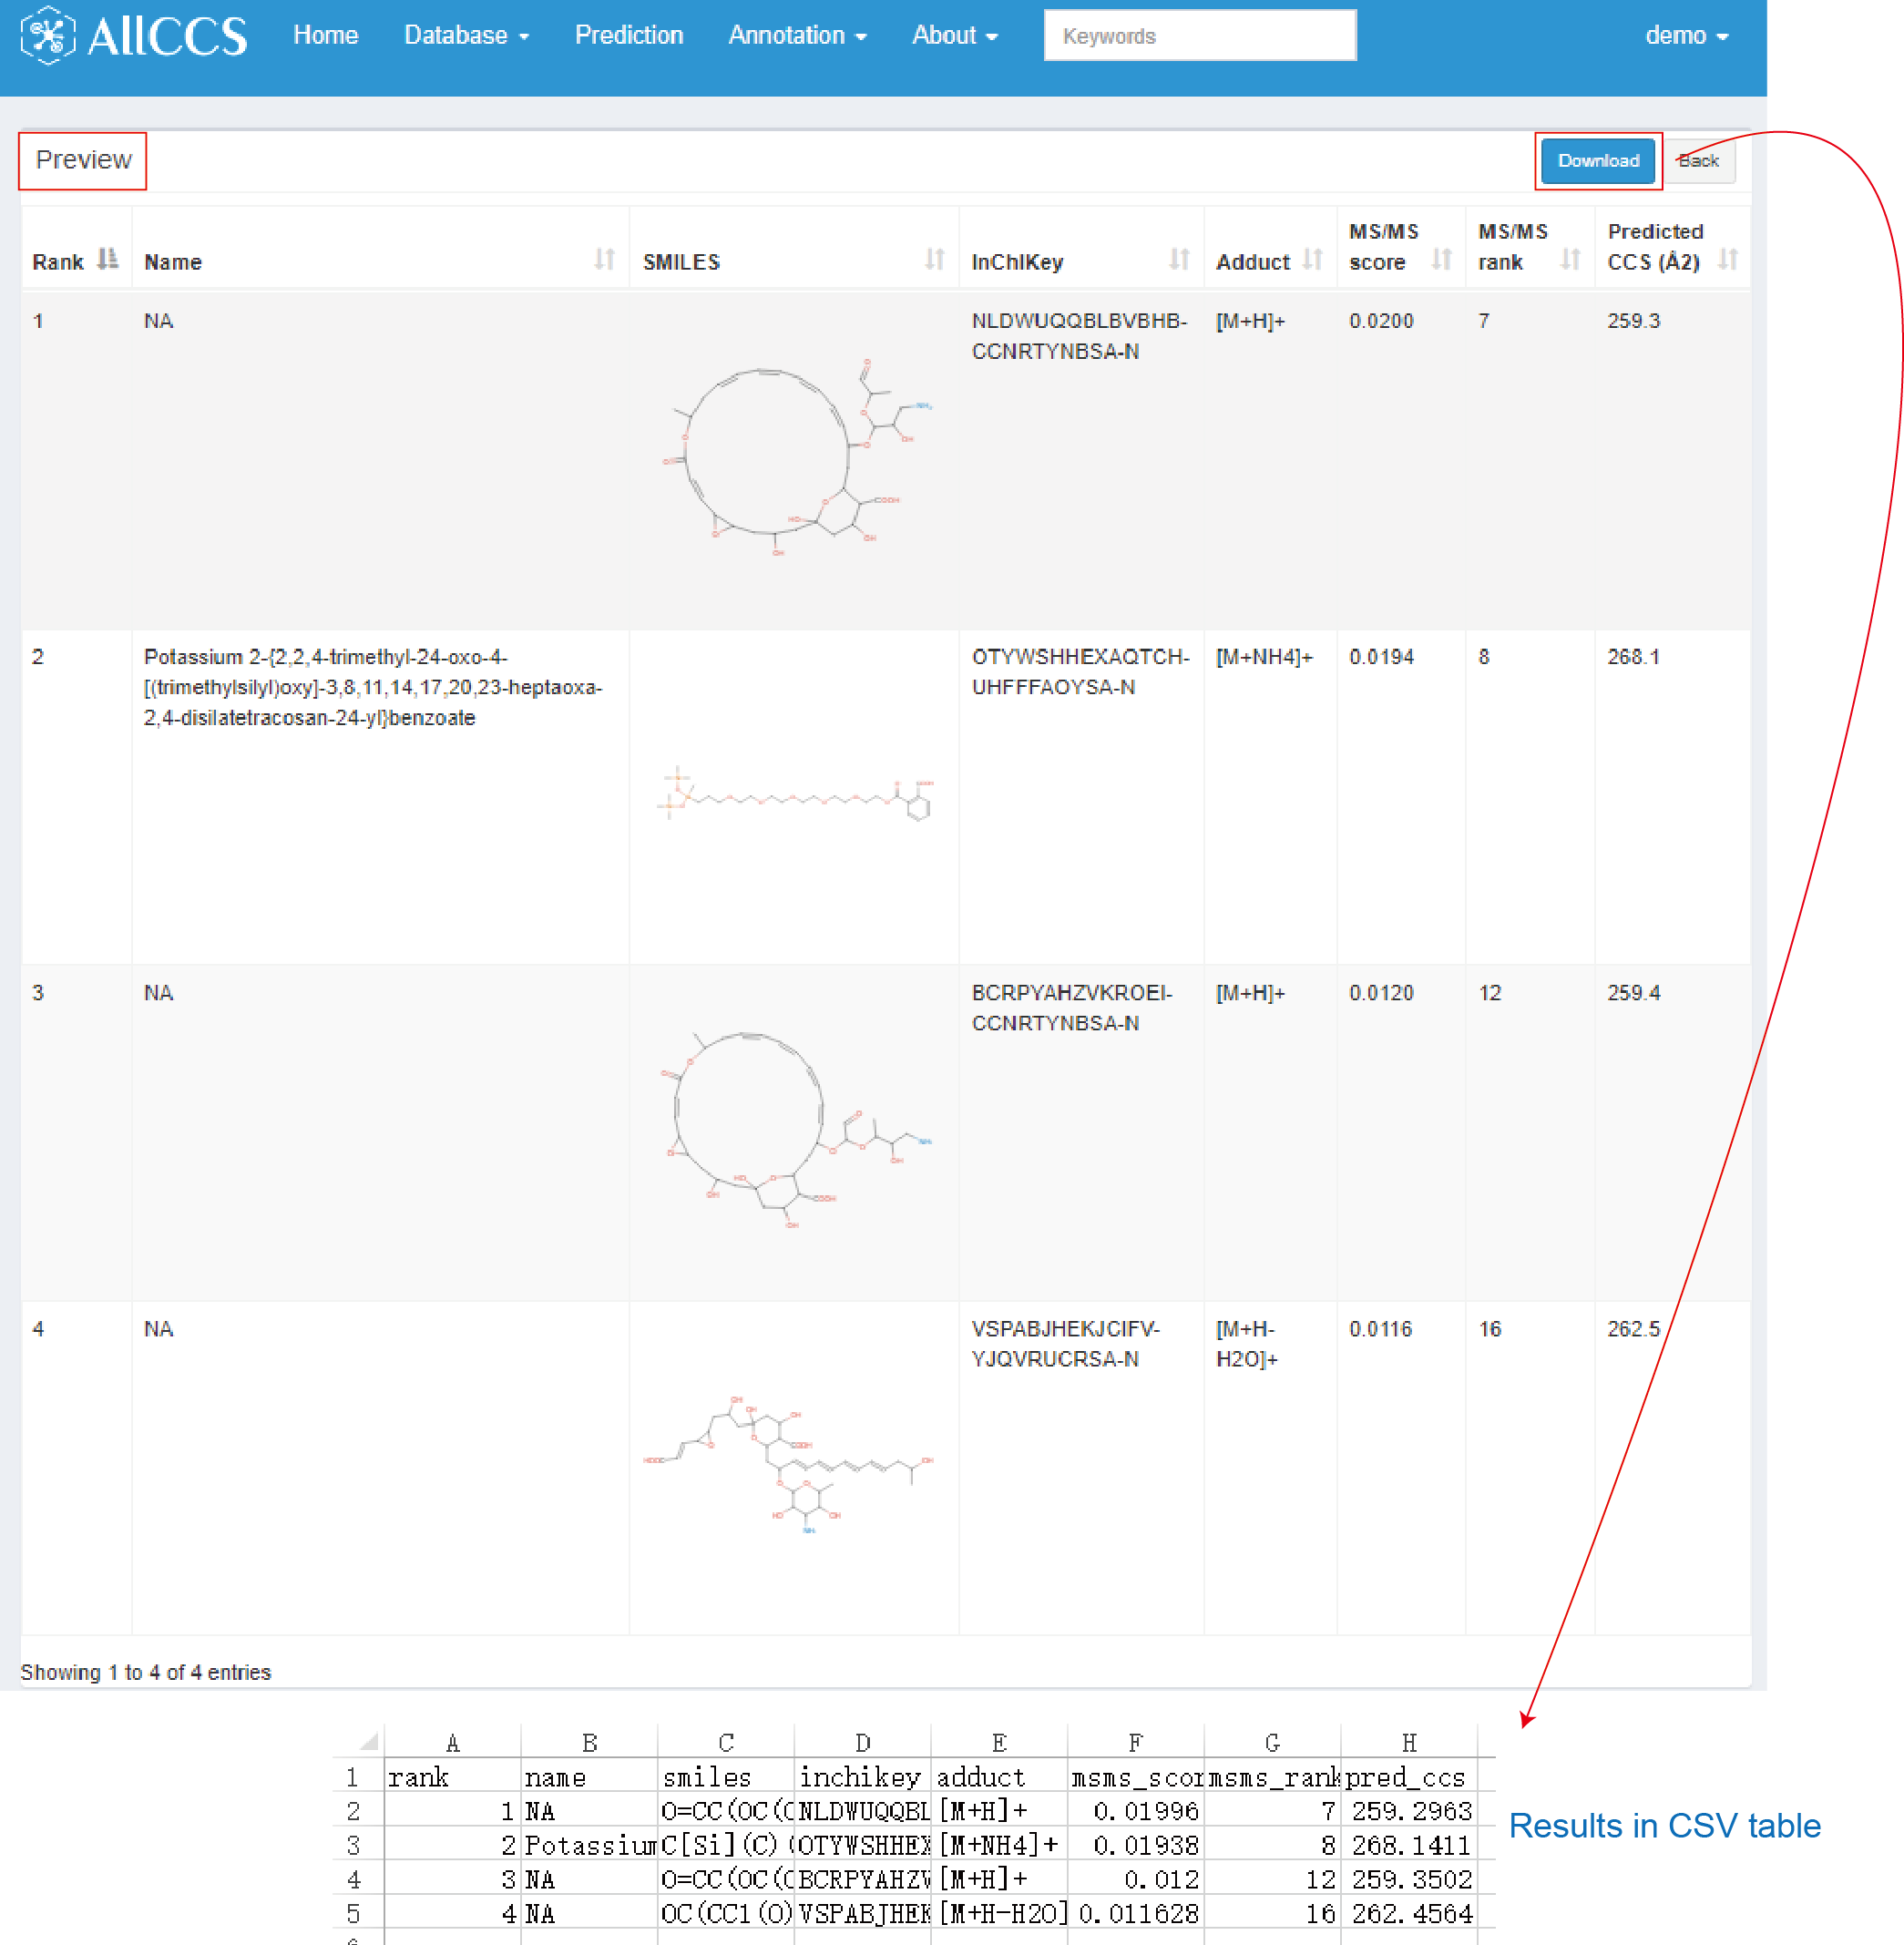
\includegraphics{images/chapter4/figure4.5candidate_rank_filter} 

}

\caption{CCS filtering result of candidates}\label{fig:figure4d5}
\end{figure}

\subsubsection{CCS scoring}\label{chapter4d2d3d2}

The results generated with CCS scoring function are similar with results
from CCS filtering (Figure \ref{fig:figure4d6}). The difference is that
CCS scoring has two additional columns as CCS score and integrated
score.

\begin{itemize}
\tightlist
\item
  \textbf{CCS score}: CCS score generated by comparing experimental CCS
  to predicted CCS values. CCS match is scored using a trapezoidal
  function. (The detail of trapezoidal function LipidIMMS Analyzer
  \citep{reference9})
\item
  \textbf{Integrated score}: The integrated score is calculated using a
  linear weighting function according to the user-defined weight for
  each match score.
\end{itemize}

\begin{figure}

{\centering 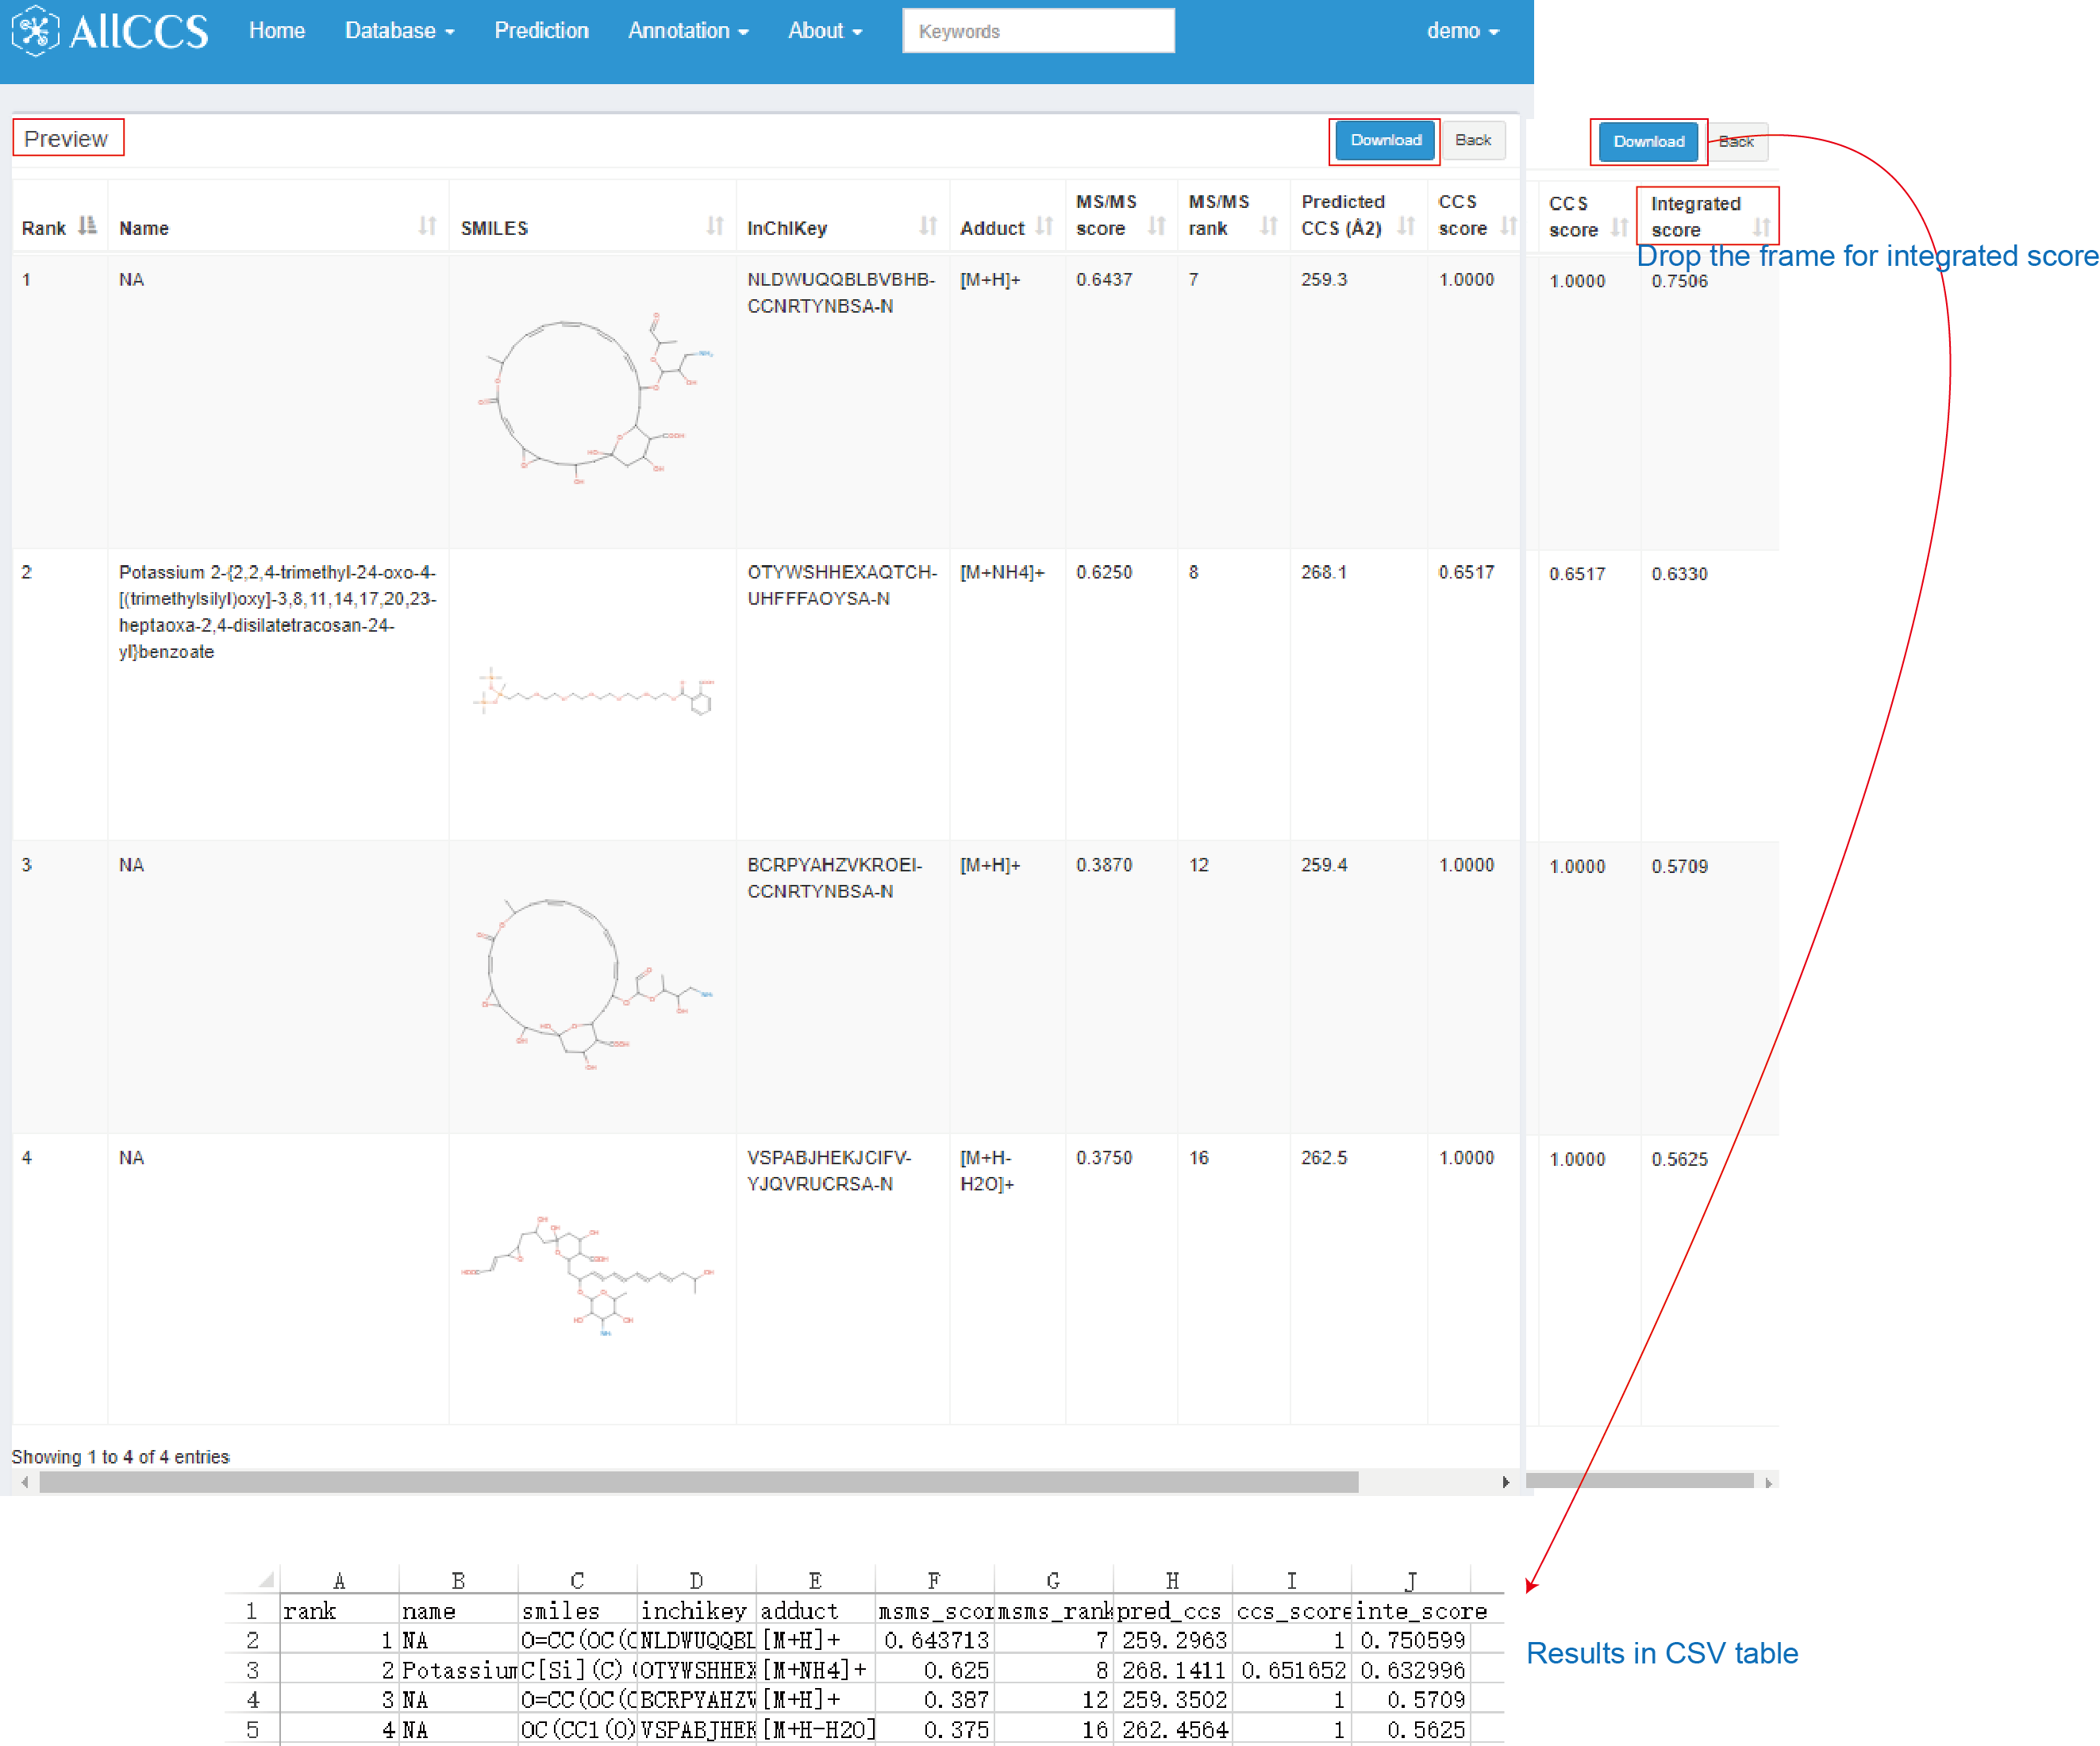
\includegraphics{images/chapter4/figure4.6candidate_rank_scoring} 

}

\caption{CCS scoring result of candidates}\label{fig:figure4d6}
\end{figure}

\bibliography{reference.bib,book.bib,packages.bib}


\end{document}
